\chapter{Incoherent and Robust Sensing Matrix Design}
\label{chap:chap4}
%
\section{Introduction}
%
In a CS system, the measurement vector $\bm{y} \in \Re^{M \times 1}$ is related to the signal of interest $\bm{x} \in \Re^{N \times 1}$ via a sensing matrix $\bm{\Phi} \in \Re^{M \times N}$ as:
%--------------------------------------------------%
\begin{equation}
\label{eq:projections_3}
     \bm{y} = \bm{\Phi}\bm{x}
\end{equation}
%--------------------------------------------------%

In this chapter, concepts from frame theory for designing incoherent tight frames are used. As defined earlier, a frame $\bm{D}$ in a real or complex $M$-dimensional Hilbert space can be represented as a sequence of $L \left(\geq M\right)$ basis vectors $\{\bm{d}_{k}\}_{k = 1}^{L}$, $\bm{d}_{k} \in \mathcal{H}^{M}$:
%-----------------------------------------------%
\begin{equation}
\label{eq:parseval_3}
 \alpha\|\bm{v}\|^{2}_{2}\leq \|\bm{D}^{T}\bm{v}\|_{2}^{2} \leq\beta\|\bm{v}\|^{2}_{2},\quad \forall\bm{v}\in\mathcal{H}^{M}
\end{equation}
%-----------------------%
where $\alpha$ and $\beta$ are positive constants. If all the frame vectors have unit $\ell_{2}$-norm i.e., $\|\bm{d}_{k}\|_{2} = 1 \, \forall k$, the frame is known as a unit norm frame (UNF). A frame is an equiangular frame if there exists a constant $c \in (0,1)$ such that $\lvert\langle \bm{d}_{i},\bm{d}_{j}\rangle\rvert = c, \forall\, i \neq j$, and $\lvert\langle \bm{d}_{i},\bm{d}_{j}\rangle\rvert = 1, \forall\, i = j$.

%---------------------------------------------------%
From the discussion on frame design in Section~\ref{subsec: Chap1_Frame}, we note the need for constructing a tight frame that is almost equiangular. We formulate an optimization problem that considers the RIP by targeting a smaller value of the RIC and a projection matrix with lower mutual coherence.

Consider the $\ell_{1}$-coherence function $\mu_{1}$, a more general concept of coherence, of a frame $\bm{D}$ defined as:
%---------------------%
\begin{equation}
    \label{eq: l1 coherence}
    \mu_{1}(s) = \underset{i\in \left[L \right]}{\max}\; \max\left\{\underset{j\in \bm{\mathcal{P}}}{\sum} \lvert\langle \bm{d}_{i},\bm{d}_{j} \rangle\rvert, \text{card}(\bm{\mathcal{P}}) = s,i \notin \bm{\mathcal{P}} \right\}
\end{equation}
%----------------------%
where $\bm{\mathcal{P}} \subset \left[L\right]$ and $1 \leq s \leq L-1$. It can be shown that $\mu \leq \mu_{1}(s) \leq s \mu$~\cite{Foucart}. Next consider Theorem 5.3 from~\cite{Foucart} stated below.
%
\begin{theorem}
\label{th: RIP_L1}
Let $\bm{D}$ be a frame with $\ell_{2}$-normalized columns and assume $s\in [L]$. For all $s$-sparse vectors $\bm{\theta}$:
%----------------------%
\begin{equation}
    \label{eq: RIP_mu_1}
     \left(1-\mu_{1}\left(s - 1\right)\right)\|\bm{\theta}\|_{2}^{2}\leq\|\bm{D}\bm{\theta}\|_{2}^{2}\leq\left(1+\mu_{1}\left(s - 1\right)\right)\|\bm{\theta}\|_{2}^{2}
\end{equation}
%----------------------%
\end{theorem}
%
In other words, for each set $\bm{\mathcal{P}} \subset [L]$ with card($\bm{\mathcal{P}}$) $\leq s$, the eigenvalues of the Gram matrix $\bm{D}_{\bm{\mathcal{P}}}^{T}\bm{D}_{\bm{\mathcal{P}}}$ lie in the interval $[(1-\mu_{1}(s-1)), (1+\mu_{1}(s-1))]$. 
%
\begin{proof}
\label{proof: RIP_L1}
Refer~\cite{Foucart} for the proof.
\end{proof}
%---------------------------------------------------%
%
\section{Proposed ETF Design Method}
%
In this chapter, the first objective is to construct a frame $\bm{D}$ which not only satisfies the equiangular property but also exhibits tightness in terms of the spectral constraint. For designing such a frame, we need to constrain the spectral and structural properties of the Gram matrix. Next, we discuss these constraints for frame design and formulate the iterative optimization problem.
%------------- off-diagonal elements ---------------%
\subsection{Structural Constraint}
%
For reduced pairwise mutual correlation, the off-diagonal elements of the Gram matrix should be close to zero and the diagonal elements should be close to unity. The structural constraint set for an ETF with unit norm vectors and pairwise inner product not larger than $\epsilon$ is given by:
%-------------------------------------------------------%
\begin{equation}
    \label{eq: Projection_set}
    \bm{\mathcal{H}}_{\epsilon} = \left\{ \bm{H}\in\Re^{L \times L};\bm{H}=\bm{H}^{T};\bm{H}_{ii}=1; \underset{i\neq j}{\max}\,\lvert \bm{H}_{ij}\rvert\leq\epsilon\right\}
\end{equation}
%----------------------------------------------------%
%
where $\epsilon\in \left(0,1\right)$ controls the search space for the desired ETF. Projecting onto the convex projection set $\bm{\mathcal{H}}_{\epsilon}$ bounds the off-diagonal elements, which in turn implies reduced mutual coherence~\cite{Elad}, as below:
%---------------------------------------------------%
\begin{equation}
    \label{eq:shrinkage_fn_4}
    S_{\bm{\mathcal{H}}_{\epsilon}}(\bm{G}):\underset{(i\neq j)}{\bm{G}_{ij}} =
    \begin{cases}
      \bm{G}_{ij} & \lvert \bm{G}_{ij}\rvert \leq \epsilon \\
      \text{sign}(\bm{G}_{ij})\cdot\epsilon & \quad \text{otherwise}
    \end{cases}
\end{equation}
%
%-----------------------------------------------%
%------------ Problem 1 ------------------------%
%------------ Eigen values ---------------------%
\subsection{Spectral Constraint}
%
The structural constraint helps in reducing the mutual correlation but such frames are far from being tight. The shrinkage function~\eqref{eq:shrinkage_fn_4} results in a Gram matrix $\bm{G}_{\epsilon}$ that is full-rank. To ensure tightness, we use a spectral constraint to reduce the rank of the Gram matrix to $M$ based on Theorem~\ref{th: RIP_L1}. From~\eqref{eq: RIP_mu_1} and mutual coherence measure~\eqref{eq: mu_for_frame}, the eigenvalues of the target Gram matrix should lie in the range $[(1-\mu_{1}(s-1)), (1+\mu_{1}(s-1))]$, where $\mu_{1}(s)\leq s\mu$. Thus, we design an ETF based on the sparsity level of the underlying signal and the desired mutual coherence. 

Let the eigen decomposition of $\bm{G}_{\epsilon}$ be $\bm{Q}\bm{\Lambda}\bm{Q}^{*}$, where the diagonal elements of $\bm{\Lambda}$ (i.e., the eigenvalues of $\bm{G}_{\epsilon}$) are sorted in descending order and $\bm{Q}^{*}$ is the conjugate transpose of $\bm{Q}$. For the spectral constraints, in terms of restricting the eigenvalues of the Gram matrix, consider a set of Gram matrices corresponding to the set of tight frames given by: 
%
%----------------------------------------------%
\begin{equation}
    \label{eq: Spectral_fn}
    \bm{\mathcal{H}}_{\bm{\mathcal{T}}}=\left\{\bm{H}\in\Re^{L\times L},\bm{H}=\bm{H}^{T},\,
    \text{and eigenvalue matrix}\, \bm{\Lambda}_{\bm{\mathcal{T}}}\right\}
\end{equation}
%-----------------------------------------------%
%-----------------------------------------------%
\begin{equation}
    \label{eq: Omega_thresh}
    \left[\bm{\Lambda}_{\bm{\mathcal{T}}}\right]_{ii} =
    \begin{cases}
      \Omega_{1} & \text{if } \lambda_{ii} < \Omega_{1}; i \leq M \\
      \Omega_{2} & \text{if }\lambda_{ii}\geq \Omega_{2}; i \leq M 
    \end{cases} 
\end{equation}
%
where the eigenvalues $\lambda_{ii}$ of the Gram matrix $\bm{G}_{\epsilon}$ are sorted in descending order and $\Omega_{1} = 1-\mu_{1}(s-1)$ and $\Omega_{2}=1+\mu_{1}(s-1)$. The sorted eigenvalues are thresholded as in~\eqref{eq: Omega_thresh} resulting in a spectrally constrained eigenvalue matrix $\bm{\Lambda}_{\bm{\mathcal{T}}} \in \Re^{M \times M}$ with $M$ non-zero eigenvalues. 

Let $\bm{Q}_{M}$ be the $L\times M$ eigenvector matrix formed from the first $M$ columns of $\bm{Q}$. The desired Gram matrix is given by $\bm{G}_{\mathcal{\bm{T}}}^{\epsilon} = (\bm{Q}_{M} \sqrt{\bm{\Lambda}_{\bm{\mathcal{T}}}}) (\bm{Q}_{M} \sqrt{\bm{\Lambda}_{\bm{\mathcal{T}}}})^{*}$, and the corresponding frame $\bm{D}_{ETF}$ is obtained as~\cite{Frame}:
%--------------------------------------------------------%
\begin{equation}
    \label{eq: Optimal_frame}
    \bm{D}_{\text{ETF}} = \sqrt{\bm{\Lambda}_{\bm{\mathcal{T}}}} \bm{Q}_{M}^{*}
\end{equation}
%----------- Algorithm ETF ----------------------------%
Thus, $\bm{D}_{\text{ETF}}$ is optimized with respect to the Gram matrix by minimizing the off-diagonal elements of the Gram matrix followed by the spectral constraint on the eigenvalues.
An iterative projection algorithm for incoherent frame design (IFD) is presented in Algorithm~\ref{Algo: Frame}. 
%---------------------------------------------------------------%
\begin{algorithm}
\SetAlgoLined
\textbf{Objective}: Design an ETF\\
\textbf{Input}: $\bm{D}_{0}$ as initialized frame matrix, $N_{\text{frame}}$ \\
\textbf{Initialization}: $t=0$\\
\While{$t \leq N_{\text{frame}}$}{
%
Project the Gram matrix $ \bm{G}_{t}= \bm{D}_{t}^{T}\bm{D}_{t} $ onto the structural constraint set $\bm{\mathcal{H}}_{\epsilon}$ using~\eqref{eq:shrinkage_fn} to obtain the new Gram matrix $\bm{G}_{\epsilon}$.\\
%
Compute the eigen decomposition of $\bm{G}_{\epsilon}=\bm{Q}\bm{\Lambda}\bm{Q}^{*}$\\
%
Project $\bm{G}_{\epsilon}$ onto the spectral constraint set $\bm{\mathcal{H}}_{\bm{\mathcal{T}}}$ by thresholding the eigenvalues using~\eqref{eq: Omega_thresh}.\\
%
Update the Gram matrix: $\bm{G}_{\bm{\mathcal{T}}}^{\epsilon} = \bm{Q}_{M} \bm{\Lambda_{\mathcal{T}}}\bm{Q}_{M}^{*}$\\
%
Compute ETF for the Gram matrix $\bm{D}_{t+1}=\sqrt{\bm{\Lambda}_{\bm{\mathcal{T}}}} \bm{Q}_{M}^{*}$\\
%
$t=t+1$}
%
\textbf{Output}: Frame matrix $\bm{D}_{\text{ETF}}=\bm{D}_{t-1}$
\caption{Incoherent frame design (IFD)}
\label{Algo: Frame}
\end{algorithm}

%------------------------------------------------------%
%------------- Remark ---------------------------------%

\noindent\textbf{Remarks}: 
%
\begin{itemize}
%
\item The ``shrinkage'' process in ~\eqref{eq:shrinkage_fn} is similar to that in~\cite{Elad} as the structural constraint set $\bm{\mathcal{H}}_{\epsilon}$ limits the pairwise correlation.
%
\item In this work, the tightness constraint for the frame is characterized by restricting the eigenvalues using the set $\bm{\mathcal{H}}_{\bm{\mathcal{T}}}$ rather than being defined by a tightness constant such as $(L/M)$~\cite{Frame, Eva_frame} or $\left(\frac{1}{M}\sum_{i=1}^{M}\lambda_{ii}\right)$~\cite{SRE_Huang} which limits the search space for the best solution. We define the search space for the frame such that the corresponding Gram matrix has eigenvalues restricted to the range $[\Omega_1,\Omega_2]$ with each eigenvalue being equal to $\Omega_1$ or $\Omega_2$ as given in~\eqref{eq: Omega_thresh}.
%
\item For constructing an ETF, the IFD algorithm uses two constraint sets: $\bm{\mathcal{H}}_{\epsilon}$ for the shrinkage process and $\bm{\mathcal{H}}_{\bm{\mathcal{T}}}$ for restricting the eigenvalues. In addition, it is required to construct an ETF with Gram matrix whose diagonal elements are unity with rank constrained properties as given below:
%
%-------------------------------------%
\begin{equation*}
    \label{eq: two_sets}
    \begin{split}
    & \bm{\mathcal{H}}_{\text{diag}} = \{\bm{H} \in \Re^{L \times L}: \bm{H}=\bm{H}^{T}, h_{ii}=1, \forall i=1,\dots,L\}\\
    & \bm{\mathcal{H}}_{\text{rank}} = \{\bm{H} \in \Re^{L \times L}: \bm{H}=\bm{H}^{T}, \text{ rank}(\bm{H})=M \}
    \end{split}
\end{equation*}
%--------------------------------------%
%
\item Alternating projections do not increase the distance between consecutive iterates. However, it may not result in a solution which is closest to the constraint sets~\cite{Frame}~\cite{Lewis_convergence}. The solution with respect to these constraint sets results in an ETF, and the non-increasing nature of the cost function $\|\bm{D}_{t}^{T}\bm{D}_{t} - \bm{G}^{\epsilon}_{\bm{\mathcal{T}}}\|_{F}^{2}$ is guaranteed ensuring convergence of the IFD algorithm. Thus, IFD will converge with a random initialization $\bm{D}_{0}$, but it does not guarantee convergence to a global optimal solution.
%
\item There are extensions of the alternating projection method that have considered non-convex constraint sets such as $\bm{\mathcal{H}}_{\text{rank}}$ and $\bm{\mathcal{H}}_{\bm{\mathcal{T}}}$. In~\cite{Alternating_Lewis}, alternating projections on manifolds has been studied and convergence is proved for two smooth manifolds which intersect transversally. In~\cite{Lewis_convergence}, authors considered alternating projections on two non-convex sets and the method converges locally to a point of intersection at a linear rate. 
%
\item The constraint sets $\bm{\mathcal{H}}_{\epsilon}$ and $\bm{\mathcal{H}}_{\text{diag}}$ are convex, and $\bm{\mathcal{H}}_{\text{rank}}$ and $\bm{\mathcal{H}}_{\bm{\mathcal{T}}}$ are smooth manifolds. Hence, the convergence results for the alternating minimization approach cannot be applied here directly~\cite{Proj_jonathan}. The convergence proof of alternating projections with more than two constraint sets, some of which are non-convex, is still an open problem. Thus, we discuss the convergence of the IFD algorithm mainly based on simulations.
%
\end{itemize}

\section{Robust Sensing Matrix Design}
%
The underlying signal or data $\bm{X}$ is represented in terms of the sparsifying basis $\bm{\Psi}$ by the sparse representation coefficients $\bm{\Theta}$ with the sparse encoding error (SEE) given by $\bm{E}=\bm{X}-\bm{\Psi}\bm{\Theta}$. Depending on the sparsity level and its relationship with mutual coherence~\eqref{eq:sparse_bound}, optimized projections in~\cite{Elad,Xuprojection,Sapiro,Zelnik} are designed to reduce pairwise correlation. Sensing matrices designed in this manner have very small correlation with the transform basis, and the CS system is able to perform better than with a random sensing matrix, with $\bm{E}=0$ for exactly sparse signals. In the real world, signals are not exactly sparse and are only compressible. Thus it is not possible to learn the ground truth dictionary and even for a learned transform basis, a non-zero SEE $\bm{E}$ exists. In such scenarios, if $\bm{\Phi}$ is not designed appropriately, then the recovery performance can be adversely affected when the sensing matrix projects $\bm{E}$ onto the measurement domain. Therefore, the SEE must be taken into account while optimizing the sensing matrix. A robust CS system, where the objective is to reduce the mutual coherence and the sensing matrix energy, can be designed using the formulation below:
%
%------------------------%
\begin{equation}
    \label{eq: Objective_intro}
           \bm{\Gamma}(\bm{\Phi}, \bm{D}) =  \underset{\bm{\Phi}}{\min}\quad \|\bm{\Phi}\bm{\Psi}-\bm{D}\|_{2,1} + \gamma\|\bm{\Phi}\bm{E}\|_{F}^{2}
\end{equation}
%------------------------%
%
where $\gamma$ is the weight parameter for the encoding error, $\bm{D} = \bm{D}_{\text{ETF}}$ is the equiangular tight frame from Algorithm~\ref{Algo: Frame}, and $\|\bm{\Phi}\bm{\Psi}-\bm{D}\|_{2,1} $ is the fidelity term. Here, row-wise $\ell_{2,1}$ norm of $\bm{A}$ is given by $\|\bm{A}\|_{2,1} = \sum_{i} \sqrt{\sum_{j} |\bm{A}_{ij}|^{2}}$. In conventional methods, the squared $\ell_{2}$-norm and Frobenius norm are usually employed which tend to amplify the effect of outliers and noisy data. The $\ell_{2,1}$ norm is more robust than the Frobenius norm and squared $\ell_{2}$-norm~\cite{RSLDA, RDR}. The $\ell_{2,1}$-norm promotes row sparsity with a few non-zero rows. Thus,~\eqref{eq: Objective_intro} optimizes the sensing matrix based on the ETF while being robust to noise and outliers.

However,~\eqref{eq: Objective_intro} optimizes the sensing matrix based on the SEE $\bm{E}$, which in turn can be obtained from a large training data $\bm{X}$. This would require large memory storage and increase the computational complexity~\cite{HONG_robust}. For a learned transform basis $\bm{\Psi}$ which represents the data sparsely, the SEE energy $\|\bm{E}\|_{F}^{2}$ is small. However, when projecting the sparse error onto the measurement domain using the sensing matrix $\bm{\Phi}$, $\|\bm{\Phi}\bm{E}\|_{F}$ can become very large if the projection matrix is not designed appropriately. This in turn affects the reconstruction accuracy of the CS system adversely. Based on the norm consistency property, we have $ \|\bm{\Phi}\bm{E}\|_{F} \leq \|\bm{\Phi}\|_{F}\|\bm{E}\|_{F}$. This implies that if $\bm{\Phi}$ is optimized appropriately, then a small $\|\bm{\Phi}\|_{F}$ would result in a smaller projected error $\|\bm{\Phi}\bm{E}\|_{F}$~\cite{HONG_robust}. Moreover, when a large training data set is used to represent the class of underlying signals, energy in the corresponding SEE $\bm{E}$ is expected to be spread evenly across the columns. Therefore, the resultant SEE $\bm{E}$ can be viewed as an additive white Gaussian noise.
Based on the above discussion, we can minimize $\|\bm{\Phi}\|_{F}$ while targeting the SEE and construct an optimized sensing matrix using the reformulated objective function given below:
%
%----------------------------%
\begin{equation}
    \label{eq: IR-PMD_objective}
   \bm{\Gamma}(\bm{\Phi}, \bm{D}) = \underset{\bm{\Phi}}{\min}\quad \|\bm{\Phi}\bm{\Psi}-\bm{D}\|_{2,1} + \gamma \| \bm{\Phi} \|_{F}^{2}
\end{equation}
%----------------------------%
%
Minimizing $\|\bm{\Phi}\|_{F}$ directly not only makes the algorithm independent of the training data $\bm{X}$ and the SEE $\bm{E}$ but is applicable for any CS system as long as a learned dictionary $\bm{\Psi}$ is available. Further, to allow sensing matrix energy to be adaptively minimized with respect to the reconstruction fidelity, we introduce a weight matrix $\bm{W}$. The proposed incoherent and robust projection matrix design (IR-PMD) is reformulated as 
%------------------------------------%
\begin{equation}
    \label{eq: IR-pmd_final_obj}
    \bm{\Gamma}(\bm{\Phi}, \bm{D}) = \underset{\bm{\Phi}}{\min}\quad \|\bm{\Phi}\bm{\Psi}-\bm{D}\|_{2,1} + \gamma\|\sqrt{\bm{W}}\bm{\Phi}\|_{F}^{2}
\end{equation}
%------------------------------------%
%
where $\sqrt{\bm{W}}$ is a diagonal matrix whose elements are adapted based on $\bm{\Phi}$, and are given by:
%
\begin{equation}
    \label{eq: Define_W}
   % \color{blue}
    w_{ii} = \frac{1}{2\|\left[\bm{\Phi}\bm{\Psi}-\bm{D}\right]^{i}\|_{2}}
\end{equation}
%
Here $\left[\bm{\Phi}\bm{\Psi}-\bm{D}\right]^{i}$ is the $i^{\text{th}}$ row of $(\bm{\Phi}\bm{\Psi}-\bm{D}$), and we let $w_{ii} = \frac{1}{2 \| \left[\bm{\Phi} \bm{\Psi} - \bm{D} \right]^{i} \|_{2} + \varepsilon }$ when $\| \left[\bm{\Phi}\bm{\Psi}-\bm{D}\right]^{i}\|_{2} = 0$, where $\varepsilon$ is a small constant. The term $\|\sqrt{\bm{W}}\bm{\Phi}\|_{F}^{2}$ minimizes the sensing matrix energy weighted by $\left(\bm{\Phi}\bm{\Psi}-\bm{D}\right)$ and also aids in obtaining a stable optimal solution. A large error term $\|\left[\bm{\Phi}\bm{\Psi}-\bm{D}\right]^{i}\|_{2}$ results in a small weight $w_{ii}$ for the corresponding row of $\bm{\Phi}$ and vice versa. Hence, the elements of $\bm{\Phi}$ with lower fidelity error have a greater weight or impact on the sensing matrix optimization.
%-------------------------------------------------%
\subsection{Solving the Optimization Problem}
%--------------------------------------------------%
We propose an iterative procedure to construct the ETF $\bm{D}$ and optimize the sensing matrix $\bm{\Phi}$ alternately. At each iteration, ETF is constructed using the sensing matrix from the previous iteration via the IFD algorithm and then $\bm{\Phi}$ is optimized for the designed ETF. Using the frame $\bm{D}$ obtained from the IFD algorithm, the solution to~\eqref{eq: IR-pmd_final_obj} gives an optimized sensing matrix. For solving~\eqref{eq: IR-pmd_final_obj}, we transform the problem as:
%-------------------------%
\begin{equation}
    \label{eq: IR_pmd_easy}
  \underset{\bm{\Phi}}{\min}\quad \| \sqrt{\bm{W}} (\bm{\Phi}\bm{\Psi} - \bm{D}) \|_{F}^{2} + \gamma \| \sqrt{\bm{W}} \bm{\Phi} \|_{F}^{2}
\end{equation}
%
where $\bm{W}$ is a diagonal matrix defined in~\eqref{eq: Define_W}. 

Next, let $\sqrt{\bm{W}} \bm{\Phi} = \overline{\bm{\Phi}} \in \Re^{M \times N}$ and $\sqrt{\bm{W}} \bm{D} = \overline{\bm{D}} \in \Re^{M \times L}$. Then, we can rewrite~\eqref{eq: IR_pmd_easy} as:
%
%---------------------------%
\begin{equation}
  \label{eq: IR_pmd_final_new}
    \underset{\overline{\bm{\Phi}}}{\min}\quad \|\overline{\bm{\Phi}}\bm{\Psi} - \overline{\bm{D}}\|_{F}^{2} + \gamma\|\overline{\bm{\Phi}}\|_{F}^{2}
\end{equation}
%
To update $\bm{\overline{\Phi}}$ and eventually $\bm{\Phi}$, we differentiate the objective function in~\eqref{eq: IR_pmd_final_new} with respect to $\overline{\bm{\Phi}}$. The derivative with respect to $\bm{\overline{\Phi}}$ is given as:
%
%------------------------------%
\begin{equation}
    \label{eq: IRPMD_grad}
    \triangledown_{\overline{\bm{\Phi}}} \varrho(\overline{\bm{\Phi}}) = 2(\overline{\bm{\Phi}} \bm{\Psi} - \overline{\bm{D}}) \bm{\Psi}^{T} + 2 \gamma \overline{\bm{\Phi}}
\end{equation}
%
We can update $\overline{\bm{\Phi}}$ by setting the derivative to zero to obtain the following closed form expression:
%
\begin{equation}
    \label{eq: Phi_bar_define}
    \overline{\bm{\Phi}} = \overline{\bm{D}}\bm{\Psi}^{T} (\bm{\Psi}\bm{\Psi}^{T} + \gamma \bm{I}_{N})^{-1}
\end{equation}
%
where $\bm{I}_{N} \in \Re^{N \times N}$ is the identity matrix. Finally, the optimized sensing matrix $\bm{\Phi}$ can be obtained as:
%
\begin{equation}
    \label{eq: Phi_define}
    \bm{\Phi} = \left(\sqrt{\bm{W}}\right)^{-1}\overline{\bm{\Phi}}
\end{equation}
%
The main steps of the incoherent and robust projection matrix design (IR-PMD) algorithm are summarized in Algorithm~\ref{Algo: IR-PMD}.
%
\begin{algorithm}
\caption{Incoherent and robust projection matrix design (IR-PMD)}
\label{Algo: IR-PMD}
\begin{algorithmic} 
\REQUIRE $\bm{\Psi}$, $N_{SE}$
\STATE \textbf{Initialization}: $t=1$, $\bm{W}_{0}= \bm{I}_{m \times m}$ and $\bm{\Phi}_{0}$ randomly. 
\STATE  $t=0$
\WHILE{$t \leq N_{\text{SE}}$}
%
\STATE Compute the frame $\bm{D}_{t-1} = \bm{\Phi}_{t-1} \bm{\Psi}$ and corresponding Gram matrix $\bm{G}_{t-1}$
%
\STATE Construct ETF $\bm{D}_{t}$ using IFD algorithm~\ref{Algo: Frame}.
\STATE Update $\bm{W}_{t}$ using~\eqref{eq: Define_W} 
\STATE Update $\overline{\bm{\Phi}}_{t}$ using~\eqref{eq: Phi_bar_define}
\STATE Update $\bm{\Phi}_{t}$ using~\eqref{eq: Phi_define}
\STATE $t=t+1$
\STATE \textbf{Output}: Sensing (or projection) matrix $\bm{\Phi}=\bm{\Phi}_{t-1}$
\ENDWHILE
\STATE Frame matrix $\bm{D}_{\text{ETF}}=\bm{D}_{t-1}$
\end{algorithmic}
\end{algorithm}

%----------------------------------------------------------------%

\noindent\textbf{Remarks}: 
\begin{itemize}
%
\item Different from the approaches in~\cite{HONG_robust,HONG_sparse} which optimize $\bm{\Phi}$ based on the Gram matrix, IR-PMD algorithm optimizes the projection matrix based on the ETF designed via the IFD algorithm to ensure it is close to the target frame. This approach is more intuitive and computationally efficient.
%
\item IR-PMD algorithm employs the $\ell_{2,1}$-norm to ensure robustness of the optimized sensing matrix to outliers. The $\sqrt{\bm{W}}$ factor accounts for the reconstruction error while minimizing the sensing matrix energy.
%
\item The term $\|\sqrt{\bm{W}}\bm{\Phi}\|_{F}$ leads to a reduced sensing matrix energy while $\|\bm{\Phi}\bm{\Psi}-\bm{D}\|_{2,1}$ determines the fidelity of the approximation. The sensing matrix is optimized based on a target frame that possesses reduced mutual coherence and tightness properties, while also ensuring robustness to the encoding error. 
%
\item Key difference between the proposed IR-PMD algorithm and the approaches in~\cite{SRE_Huang,HONG_sparse,HONG_robust} is the introduction of the weighted penalty term and the $\ell_{2,1}$-norm which ensures robustness to the sparse encoding error. In addition, the cost function in~\cite{SRE_Huang} depends on the training data matrix $\bm{X}$ which tends to be very large, imposing a large memory (or storage) and computational cost on the method. The cost function in our proposed method is dependent on $\bm{\Phi}$ and $\bm{D}$ which is much more efficient in terms of memory and computations.
%
\item  The proposed IR-PMD framework is presented as a flowchart in Fig.~\ref{Fig: IR_PMD_Flow chart}. 
\end{itemize}
%
%
\begin{figure}
\centering
\scalebox{.9}{    \begin{tikzpicture}

%\draw [ thick]  (-4,0.5) rectangle (4,-8);

%\tikzstyle{every node}=[font=\small]
\tikzstyle{every node}=[font=\scriptsize]

\tikzstyle{startstop} = [rectangle, rounded corners, text centered, draw=black, fill=red!20]
\tikzstyle{io} = [trapezium, trapezium left angle=70, trapezium right angle=110,text width=5.2cm, text centered, draw=black, fill=blue!20]
\tikzstyle{process} = [rectangle, text centered, draw=black, fill=orange!20]
\tikzstyle{decision} = [diamond, text centered, draw=black, fill=green!20]
\tikzstyle{arrow} = [thick,->,>=stealth]

\node (start) [startstop] {\textbf{Given}: \begin{tabular}{l} Training data matrix $\bm{X}$;\\ Sparsifying basis $\bm{\Psi}$; \\ Maximum number of iterations $N_{SE}$; 
\end{tabular}};
\node (in1) [io, below of=start,node distance=1.4cm] {\textbf{Initialize}: $t=1$, Sensing matrix $\bm{\Phi}_{0}$ randomly, $\bm{W}_{0}=\bm{I}_{m\times m}$, parameter $\gamma$};

\node (pro1) [process, below of=in1,node distance=1.2cm] {  \textbf{Compute:} \begin{tabular}{l} Frame $\bm{D}_{t-1}$ and corresponding Gram matrix $\bm{G}_{t-1}$\end{tabular}};

\node (pro2b) [process, below of=pro1, node distance=1.2cm] { % xshift=2.5cm
\begin{tabular}{l} Update the weight matrix $\bm{W}_{t}$ \\
Update the sensing matrix $\bm{\Phi}_{t}$\end{tabular}};

\node (dec1) [decision, below of=pro2b, node distance=1.5cm,xshift=-3.5cm] {$t\leq N_{SE}$};

\node (out1) [io, below of=dec1,node distance=1.5cm, xshift=3.2cm] { \textbf{Output}: \begin{tabular}{l}  Frame matrix $\bm{D}_{\text{ETF}}=\bm{D}_{t-1}$\\ Sensing matrix $\bm{\Phi}=\bm{\Phi}_{t-1}$ \end{tabular}};

\draw [arrow] (start) -- (in1);
\draw [arrow] (in1) -- (pro1);
\draw [arrow] (pro1)  --  (pro2b);

\draw [arrow]  (pro2b) -| (dec1);
\draw [arrow] (dec1) -|  (pro2b);
%\draw[arrow](dec1) -| (pro2b)
%\draw [arrow] (dec1) -|  (out1);

\node (v1) at (-3.5,-6.07) {};
\node (v2) at (-3.08,-6.9) {};
\draw [arrow] (v1) |- (v2);
%\draw  [thick] (v1) edge (v2);
\node (v3) at (-2.9, -6.9){};
\node (v4) at (-3.5, -6.0){};
%\draw [arrow] (v4) |- (v3);
%\node (v2) at (-2.4,-3.61) {};
%\node (v1) at (-2.4,-2.86) {};
%\draw  [arrow] (v1) -- (v2);
%\node (v3) at (-3.38,-6.99) {};
%\node (v4) at (-3.38,-3.4) {};
%\draw  [arrow] (v3) -- (v4);
%\node (v6) at (-3.52,-4.1) {};
%\node (v5) at (-2.88,-4.1) {};
%\draw  [thick] (v5) edge (v6);
%\draw  [arrow] (-2.4,-4.7) -- (-2.4,-5.1) -- (1.13,-5.1) -- (1.13,-4.78);
\node at (-3.94,-6.50) {False};
\node at (-2.44,-4.93) {True};
\node at (-2.90,-4.0) {$t = t + 1$};
%\node at (-2.13,-3.2) {i=1};
%\node at (-1.6,-3.9) {i=i+1};
\end{tikzpicture}}
%\includegraphics[keepaspectratio,width=0.45\textwidth,trim=2 0 0 0,clip]{Flow_chart.eps}
\caption{Flowchart of the proposed IR-PMD model.}
\label{Fig: IR_PMD_Flow chart}
\end{figure}
%
We will show that optimized projections using IR-PMD are robust for real-life applications such as image compression and result in improved recovery performance even in the presence of noise. Simulation results on synthetic and real data sets presented in the next section will confirm these gains.
%
\subsection{Computational Complexity}
%
Computational complexity of the proposed sensing matrix design algorithm can be analyzed in two parts, IFD algorithm for designing the ETF and IR-PMD algorithm for optimized projections. The computationally dominant step of the IFD algorithm is the eigen decomposition of the Gram matrix which has complexity $\mathcal{O}\left(L^3\right)$. For IR-PMD, two steps involve matrix inversion. For updating $\overline{\bm{\Phi}}$ using~\eqref{eq: Phi_bar_define}, computational complexity of the matrix inversion is $\mathcal{O}\left(N^{3}\right)$ and the cost of matrix multiplication is $\mathcal{O}\left(M N^{2}\right)$. Hence, the overall cost for updating $\overline{\bm{\Phi}}$ is $\mathcal{O}\left(N^{3}\right)$. To update $\bm{\Phi}$, cost of matrix inversion of $\sqrt{\bm{W}}$ is $\mathcal{O}\left(M^{3}\right)$. In~\cite{SRE_Huang}, the computational cost of updating $\bm{\Phi}$ with $J$ signals in the training data set is dominated by eigen decomposition whose complexity is $\mathcal{O}\left(\min\left(N(L+J)^{2},N^{2}(L+J)\right)\right)$ which is larger than the cost of the proposed approach.
%
\section{Experimental Results}
\label{sec: Chapter_4_Results}
%
In this section, we evaluate the performance of IFD and IR-PMD algorithms on both synthetic and real data sets. The first set of experiments are performed on synthetic data to demonstrate the recovery performance of the various CS systems being compared. We generate a set of training signals based on the learned dictionary using the K-singular value decomposition (K-SVD) technique~\cite{KSVD} and white Gaussian noise is added for evaluating robustness of the CS systems. We also illustrate the effectiveness of optimized projections in real-world applications by considering image compression. 

In the proposed scheme, IFD algorithm allows us to design an ETF which is used as the target frame for optimizing the sensing matrix using the IR-PMD algorithm. We will demonstrate significant properties of the designed ETF such as the absolute and averaged mutual coherence. Next, we demonstrate the performance of incoherent and robust projections through reconstruction results under different conditions. In each CS system, we consider signals that are sparse with respect to a learned transform basis $\bm{\Psi}$. The performance of the proposed method will be compared with the techniques presented in~\cite{Elad,Eva_frame,Sapiro,Zelnik,CHZ,SRE_Huang}.
%
%-----------------------------------------%
%---- Synthetic data ---------------------%
\subsection{Performance Evaluation of IR-PMD Model on Synthetic Data}
%
We generate an $N \times L$ transform basis $\bm{\Psi}$ with Gaussian distributed entries, and initialize the projection matrix to an $M \times N$ random matrix $\bm{\Phi}_{0}$. This initial set up is used in each of the following CS systems for optimizing the projection matrix: $\text{CS}_{\text{XPC}}$~\cite{Xuprojection}, $\text{CS}_{\text{DCS}}$~\cite{Sapiro}, $\text{CS}_{\text{ZMRE}}$~\cite{Zelnik}, $\text{CS}_{\text{CHZ}}$~\cite{CHZ}, $\text{CS}_{\text{HZ}}$~\cite{HONG_robust}, $\text{CS}_{\text{HLZL}}$~\cite{HONG_sparse}, and  $\text{CS}_{\text{BLH}}$~\cite{SRE_Huang}. We use the author-provided source codes for all the algorithms, except $\text{CS}_\text{XPC}$ and $\text{CS}_{\text{CHZ}}$ which we have implemented. We use $\bm{\Phi}_{0}$ for $\text{CS}_{\text{rand}}$, and for $\text{CS}_{\text{Elad}}$~\cite{Elad} we use $\gamma=0.95$ to optimize the projections. 

First, we compare the performance of frame design using IFD algorithm, $\text{CS}_{\text{rand}}$, $\text{CS}_{\text{Elad}}$, and $\text{CS}_{\text{TKK}}$~\cite{Eva_frame}. For training and testing, synthetic data is generated using $\bm{\Psi}$ for both noiseless and noisy scenarios. Let $\{\bm{\theta}_{i}\}_{i=1}^{2J}$ be $s$-sparse vectors of dimension $L\times1$ where each vector is normally distributed with zero mean and unit variance. The signals $\{\bm{x}_{i}\}_{i=1}^{2J}$ are generated as:
%
%------------------------------------------------------%
\begin{equation}
    \label{eq: Signal_generation}
    \bm{x}_{i}= \bm{\Psi} \bm{\theta}_{i} + \bm{n}_{i} \triangleq \bm{x}_{i}^{*} + \bm{n}_{i}, \quad i=1,2,\dots,2J
\end{equation}
%------------------------------------------------------%
%
where $\bm{n}_{i}$ is zero-mean white Gaussian noise. The corresponding signal-to-noise ratio is denoted by SNR. Let $\bm{X}= \left[ \bm{x}_{1}, \bm{x}_{2},\dots,\bm{x}_{2J} \right]^{T}$ be the noisy signal and $\bm{X}^{*}= \left[ \bm{x}_{1}^{*}, \bm{x}_{2}^{*},\dots,\bm{x}_{2J}^{*} \right]^{T}$ be the original noise-free signal. For the noiseless scenario, we consider the original noise-free signal $\bm{x}_{i}= \bm{\Psi} \bm{\theta}_{i} \triangleq \bm{x}_{i}^{*}, i=1,2,\dots,2J$. The training and test data sets are obtained by dividing $\bm{X}$ into two equal parts i.e., $\bm{X}^{\text{test}}$ and $\bm{X}^{\text{train}}$ each of size $N\times J$. Measurement matrix $\bm{Y}=\bm{\Phi} \bm{X}^{\text{test}}$ is computed using the optimized sensing matrix $\bm{\Phi}$ obtained via the CS algorithms. In each case, OMP algorithm is used to recover the sparse signals from the measurement vectors by solving~\eqref{eq:L0_reconstruction}. The normalized mean square error (NMSE) is computed as:
%
%-----------------------------------------------------%
\begin{equation}
\label{eq: NMSE_42}
e_{r} = \frac{1}{N} \sum_{j=1}^{N} \frac{\|\bm{x}_{j}^{\text{test}}-\widehat{\bm{x}}_{j}^{\text{test}}\|_{2}^{2}}{\|\bm{x}_{j}^{\text{test}}\|_{2}^{2}} 
\end{equation}
%---------------------------------------------------%
%
where $\widehat{\bm{x}}^{\text{test}}_{j}$ is the recovered sparse signal. The mean square error (MSE) is computed as:
%
%-------------------------------------------------%
\begin{equation}
    \label{eq: MSE_error}
    \text{MSE} \triangleq \frac{1}{N \times J} \|\bm{X}^{\text{test}}-\widehat{\bm{X}}^{\text{test}}\|_{F}^2
\end{equation}
%------------------------------------------------%
%
$\widehat{\bm{x}}_{j}^{\text{test}}$ can be expressed in terms of the corresponding sparse coefficients as $\widehat{x}_{i}= \bm{\Psi} \widehat{\bm{\theta}}_{i}$ and the sparse coefficients $\widehat{\bm{\theta}}_{i}$ can be obtained by solving the OMP problem~\cite{Tropp}. The peak signal to noise ratio (PSNR) is defined as~\cite{KSVD}:
%--------------------------------------------------------%
\begin{equation}
    \label{eq: PSNR}
    \text{PSNR} \triangleq 10 \times \log_{10} \Bigg[\frac{(2^{r}-1)^{2}}{\text{MSE}}\Bigg]
\end{equation}
%--------------------------------------------------------%
where $r=8$ is the number of bits per pixel.
%---------------- Results for Convergence ------------------%
%-----------------------------------------------------------%
\subsubsection{Empirical Convergence}
%
For performance evaluation of the IFD algorithm, experiments are carried out with $M=20$, $L=120$, and sparsity $s=4$. We start with an arbitrary $M \times L$ matrix $\bm{D}$ with full rank, and the shrinkage function followed by the spectral constraint are applied iteratively resulting in a tight frame that is closest to being an incoherent matrix. We consider convergence of the alternating projections in the IFD algorithm based on the numerical results. The IFD distance measure $d_{\text{F}}\left(j\right)$ is used to study convergence of the iterative algorithm:
%----------------------------------------------------------%
\begin{equation}
    \label{eq: Mean_square_distance_44}
        d_{\text{F}}(j) = \|\bm{G}_{j} - \widetilde{\bm{G}}_{\mathcal{\bm{T}}}^{\epsilon}\|_{F}^{2}
\end{equation}
%----------------------------------------------------------%
where $\widetilde{\bm{G}}_{\mathcal{\bm{T}}}^{\epsilon}$ is the target optimal Gram matrix that belongs to the sets satisfying structural and spectral constraints and $\bm{G}_{j}$ is the designed Gram matrix at the $j^{\text{th}}$ iteration. 
%-------- Objective Function Together -------------%
\begin{figure}
\centering    
\subfigure[IFD distance measure ($d_{\text{F}}$)]{\label{fig: MSD}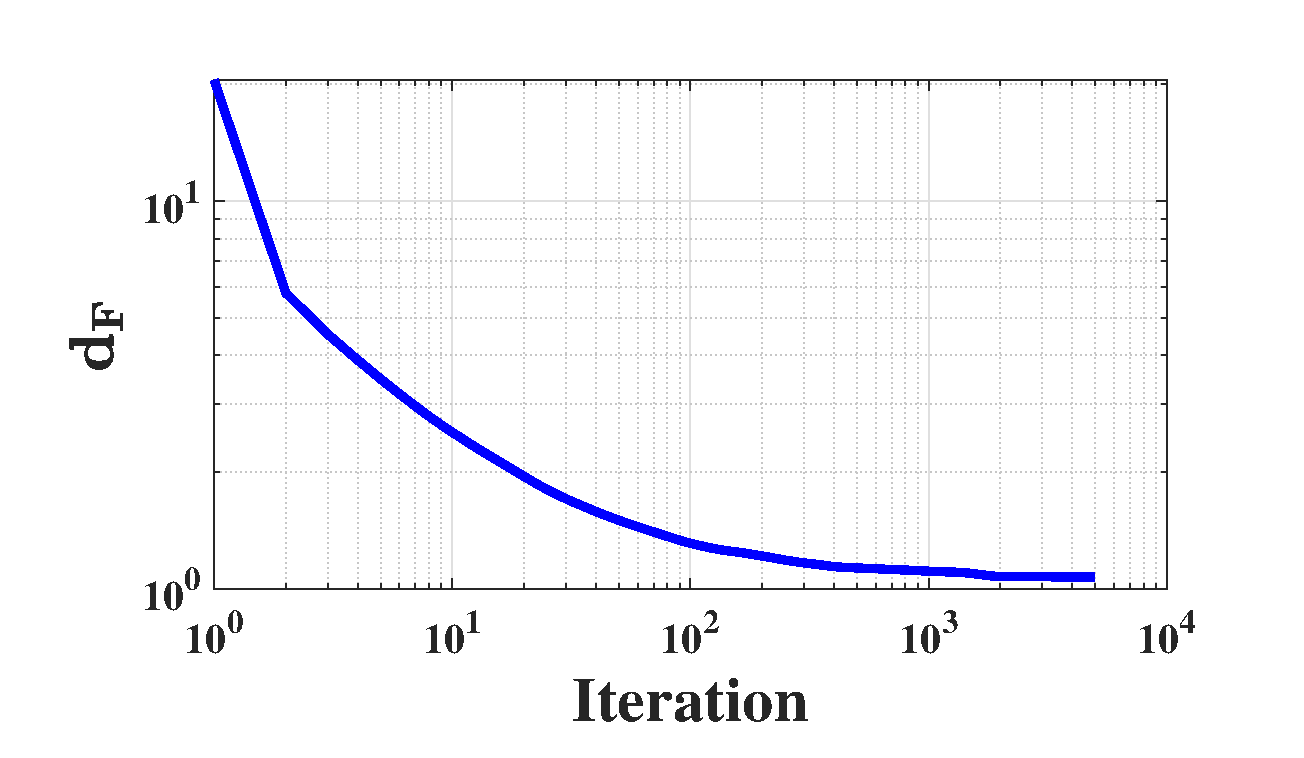
\includegraphics[keepaspectratio,width=0.47\textwidth,trim=20 5 30 25,clip]{figChap4/G_obj_loglog_g_n.eps}}
\subfigure[IR-PMD objective function~\eqref{eq: IR-pmd_final_obj}]{\label{fig:F_obj_Proj}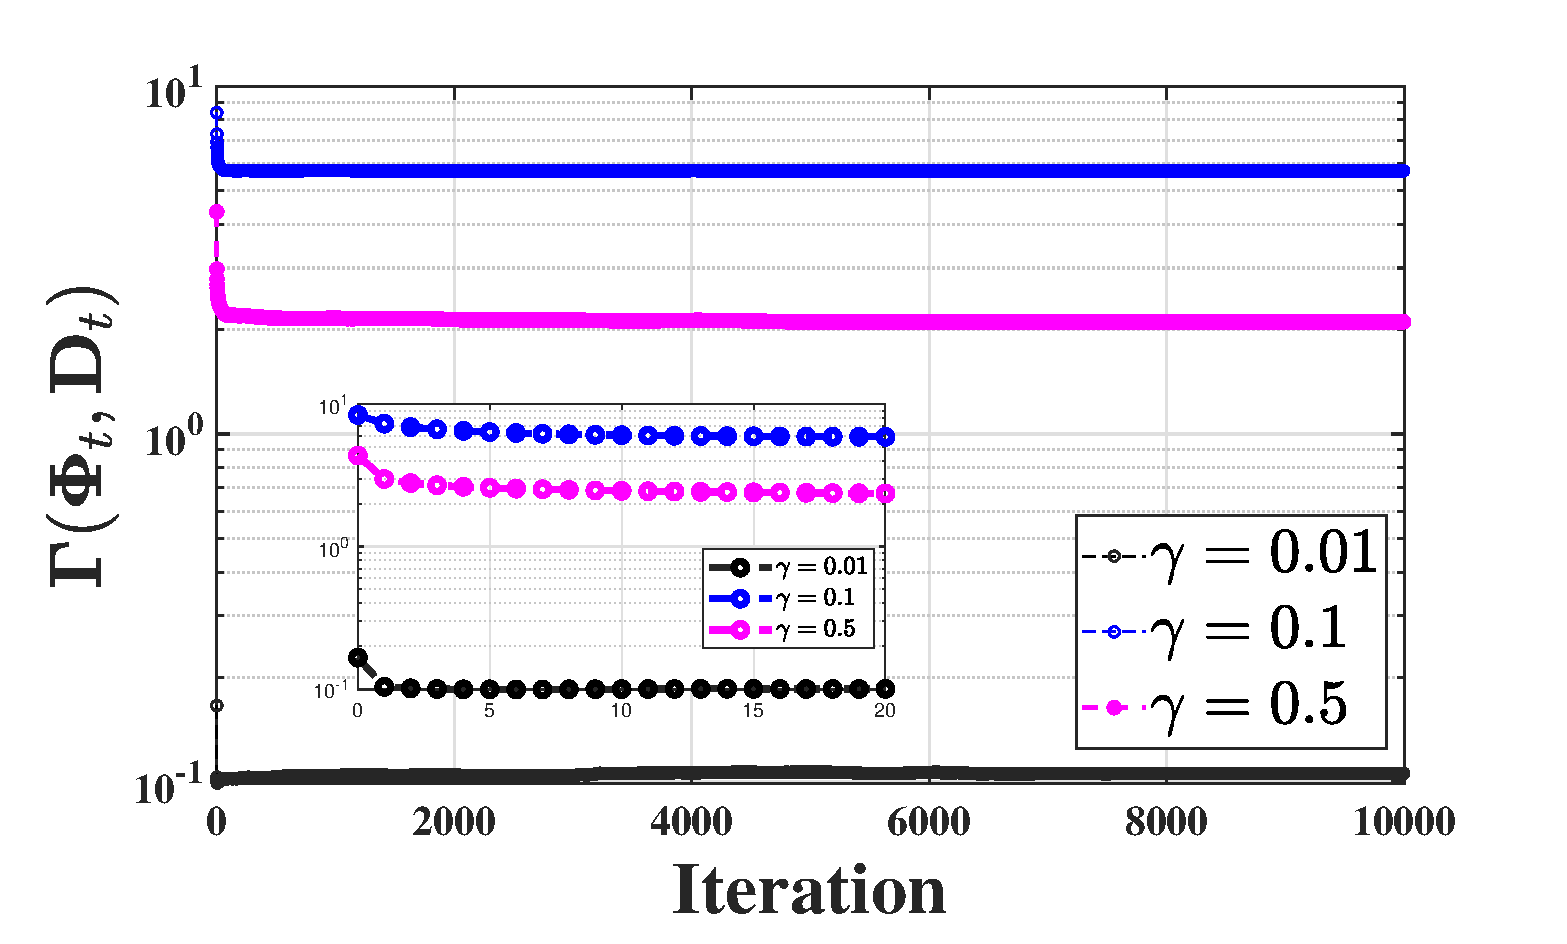
\includegraphics[keepaspectratio,width=0.47\textwidth,trim=17 5 30 25,clip]{figChap4/Syn_Obj_iter.eps}} 
\caption{Convergence behavior of IFD and IR-PMD algorithms ($M=20$, $L=120$, $N=60$, and SNR = $10$~dB).} 
\label{Fig Evolution of convergence}
\end{figure}

Fig.~\ref{fig: MSD} shows the evolution of $d_{\text{F}}$ for the IFD algorithm. It is seen that the algorithm eventually results in a frame that lies at the intersection of the constraint sets. Convergence of $d_{\text{F}}$ indicates that the frame is close to being an incoherent UNTF. For demonstrating convergence of the IR-PMD algorithm we assume $M=20$, $L=120$, $N=60$, and $N_{SE}=100$ with each experiment being repeated $1000$ times. Fig.~\ref{fig:F_obj_Proj} shows the convergence of the objective function $\bm{\Gamma}(\bm{\Phi}_t,\bm{D}_{t})$~\eqref{eq: IR-pmd_final_obj} for different values of $\gamma$ over $10000$ iterations. In order to see details of the objective function trend, the zoomed-in view of the convergence plot for different values of $\gamma$ is shown in Fig.~~\ref{fig:F_obj_Proj}.
%---------------------------%
\begin{figure}
\centering    
\subfigure[Evolution of MSE]{\label{fig: Syn_MSE_iteration}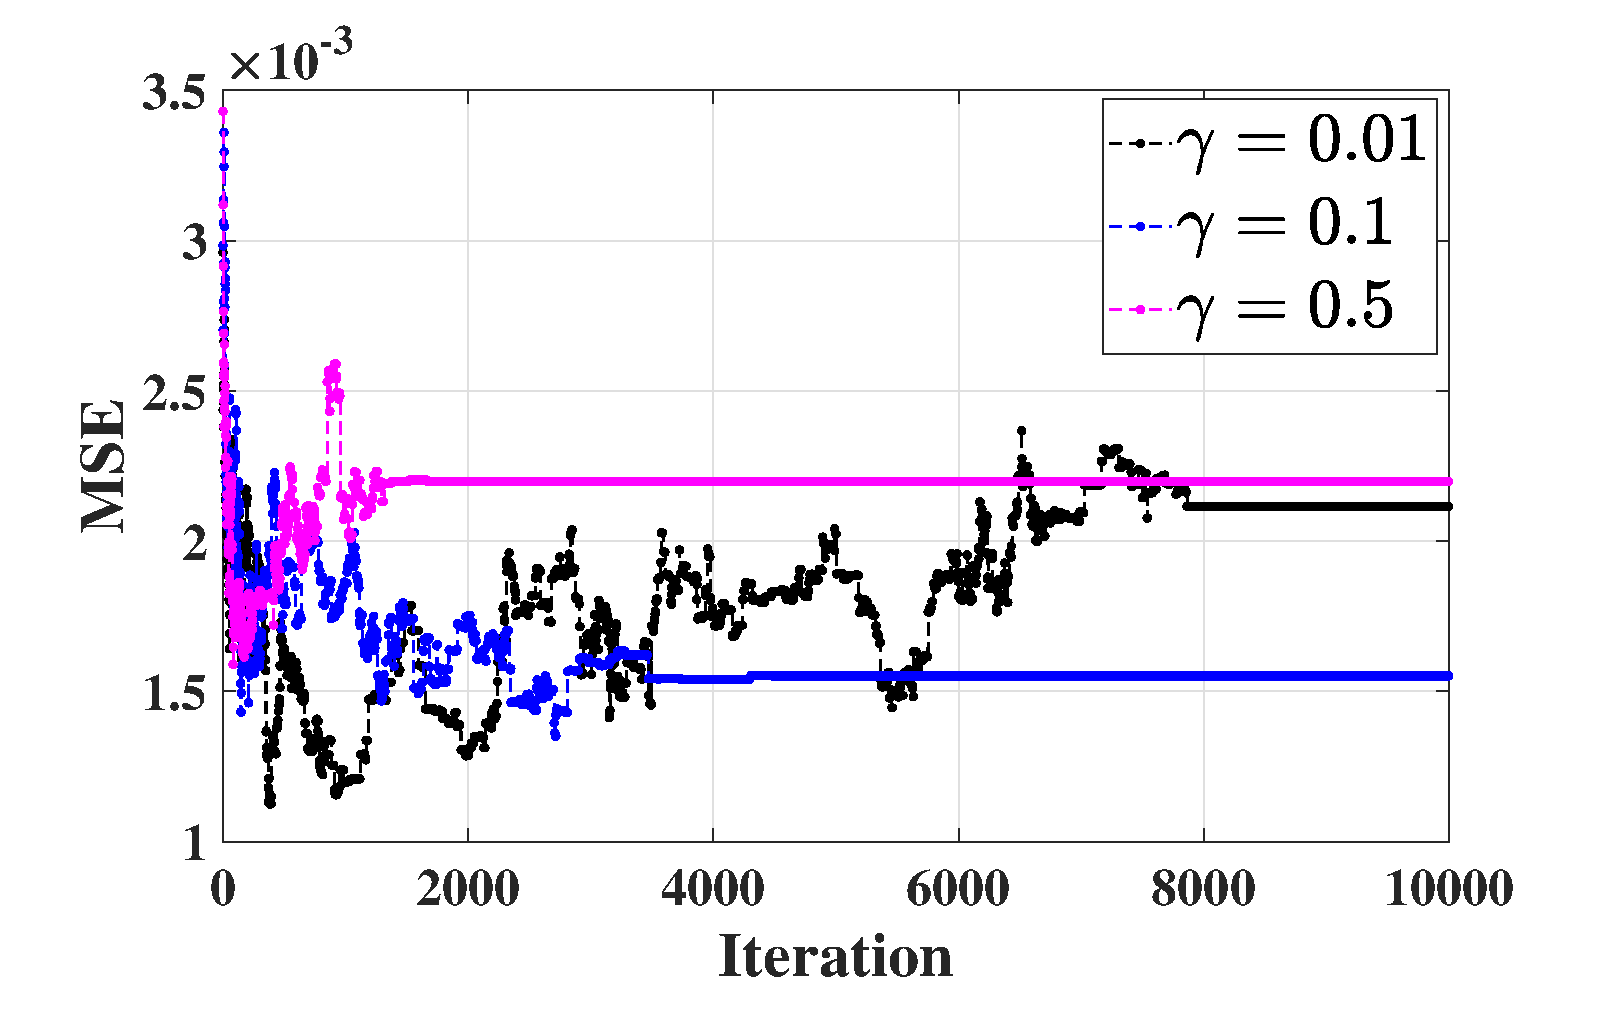
\includegraphics[keepaspectratio,width=0.47\textwidth,trim=17 5 30 2]{figChap4/Syn_MSE_Iterations.eps}}
\subfigure[Evolution of $\delta_{\bm{\Phi}}$]{\label{fig: Syn_Succ_gamma}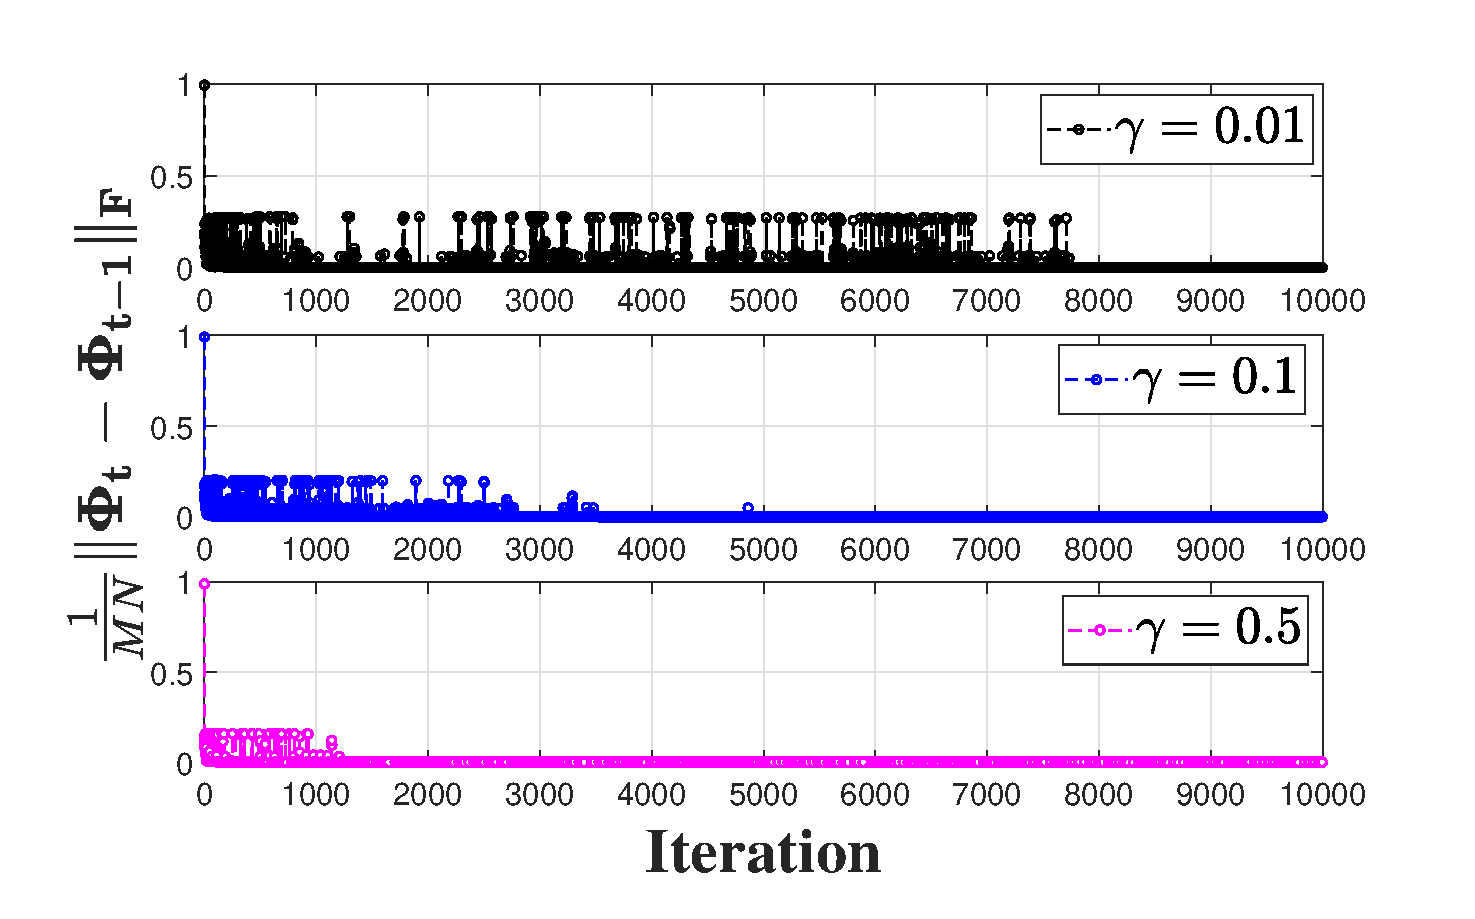
\includegraphics[keepaspectratio,width=0.47\textwidth,trim=17 5 30 2]{figChap4/Syn_Succ_iter.eps}}
\caption{Performance of IR-PMD model for synthetic data ($N = 60$, $M=20$, $L=120$, and $s=4$)} 
\label{Fig Evolution of MSE and iterate convergence}
\end{figure}
%
First, we generated the synthetic signal for the noiseless case i.e., when $\bm{n}_{i} =0, i=1,2,\dots,2J$.

Fig.~\ref{fig: Syn_MSE_iteration} shows the evolution of averaged MSE for different values of $\gamma$. Although, the objective function was seen to converge faster for smaller value of $\gamma$, MSE attains the lowest value for $\gamma = 0.1$. Note that this is the noiseless case and signals are perfectly sparse for the experiment with synthetic data, thus smaller values of $\gamma$ are able to achieve reduced pairwise correlation and improved reconstruction accuracy. Fig.~\ref{fig: Syn_Succ_gamma} shows the evolution of the iterate $\bm{\Phi}_{t}$, measured using the expression:
\begin{equation}
    \label{eq: Iterate_Phi}
    \delta_{\bm{\Phi}}(t) = \frac{1}{M N}\|\bm{\Phi}_{t} - \bm{\Phi}_{t-1}\|_{F}
\end{equation}
%
%-----------------------------------%
\begin{figure}
\centering    
\subfigure[Evolution of MSE]{\label{fig: Cal_MSE_iteration}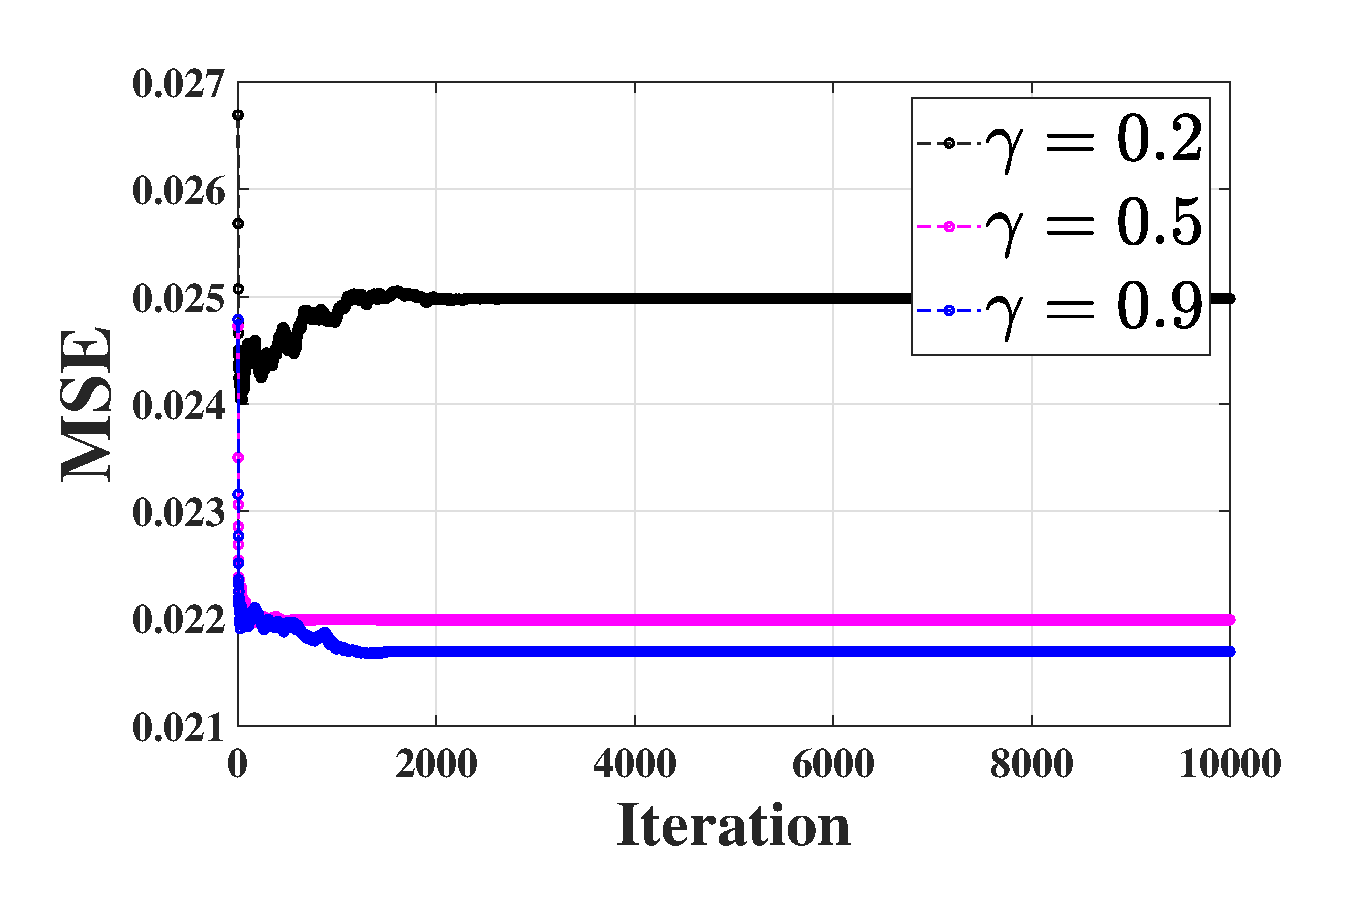
\includegraphics[keepaspectratio,width=0.47\textwidth,trim=17 5 30 25]{figChap4/Caltech_MSE_iter.eps}}
\subfigure[Averaged MSE and PSNR as a function of $\gamma$]{\label{fig:Cal_Mse_PSNR_gamma}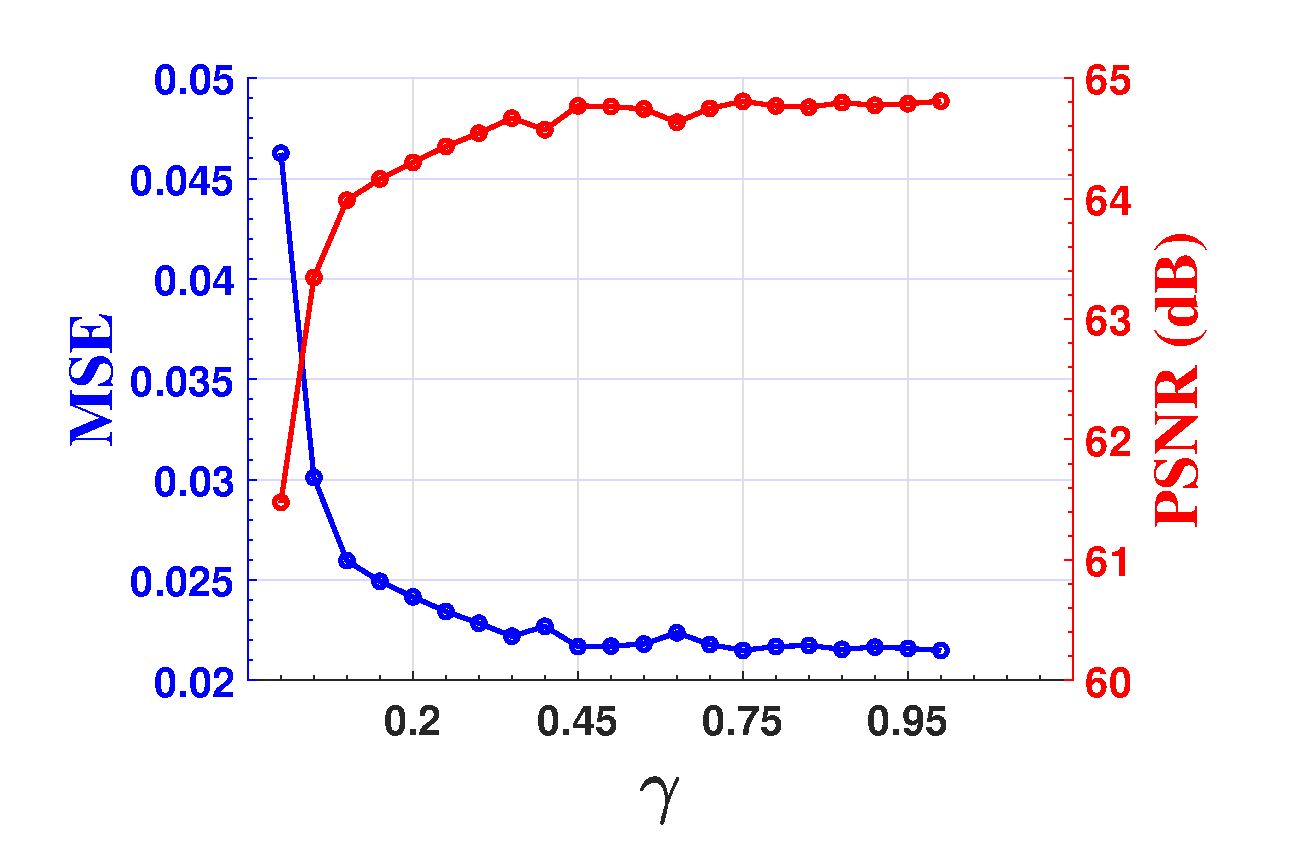
\includegraphics[keepaspectratio,width=0.47\textwidth,trim=17 5 30 25]{figChap4/Cal_MSE_PSNR_gamma.eps}}
\caption{Performance of IR-PMD model for Caltech-101 data set.} 
\label{Fig Evolution of MSE and PSNR Caltech}
\end{figure}
%------------------------------------%
It is seen that $\bm{\Phi}_{t}$ converges well for different values of $\gamma$. Next we run a similar experiment using a real data set, namely the Caltech-101 data set. Fig.~\ref{fig: Cal_MSE_iteration} shows the evolution of MSE for different values of $\gamma$. For a real data set, sparse encoding error can be significant as the underlying signal is not exactly sparse. Hence, larger value of $\gamma$ minimizes the sensing matrix energy and leads to a reduced MSE. In Fig.~\ref{fig:Cal_Mse_PSNR_gamma}, both MSE and peak signal-to-noise ratio are shown as a function of $\gamma$. It is noted that $\gamma > 0.2$, results in reduced MSE and increased PSNR. It is observed that for real images, with no additional noise the MSE decreases for larger values of $\gamma$, and for exactly sparse synthetic signals, $\gamma = 0.1$ gives improved performance. However, when the synthetic signals have a non-zero sparse encoding error, higher values of $\gamma$ minimize the sensing matrix energy with increased PSNR and reduced MSE.

%------- Evolution of Mutual Coherence -------------%
\begin{figure}
\centering
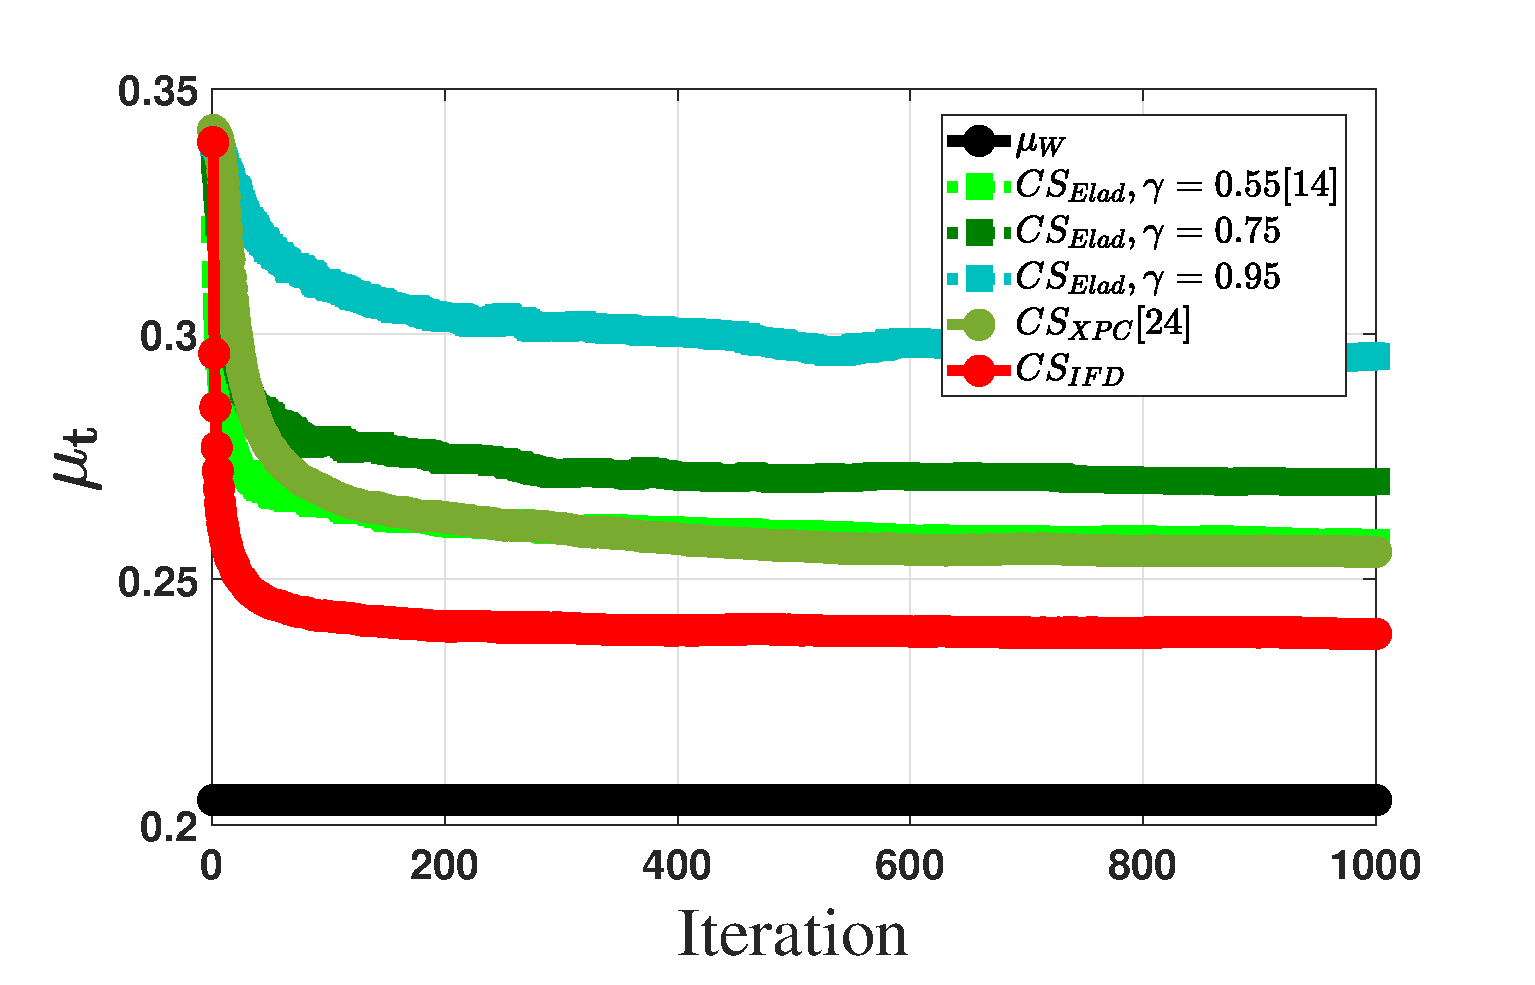
\includegraphics[keepaspectratio,width=0.50\textwidth,trim=20 0 40 25]{figChap4/M_avg_our_10.eps}
\caption{Evolution of averaged mutual coherence over 1000 trials ($M=20, L=120$, $s=4$, and SNR = $10$~dB).}
\label{fig: MU_t_frame}
\end{figure}
%----------------------------------------------------%
Fig.~\ref{fig: MU_t_frame} shows the evolution of the averaged mutual coherence over $1000$ trials for different CS techniques with SNR = $10$~dB and $s=4$. It shows that IFD results in averaged mutual coherence that is closer to the Welch bound compared to the other algorithms. 
%----------------- MU_Projection --------------------%
\begin{figure}
\centering    
\subfigure[Frame design]{\label{fig: Mu_avg_M_frame}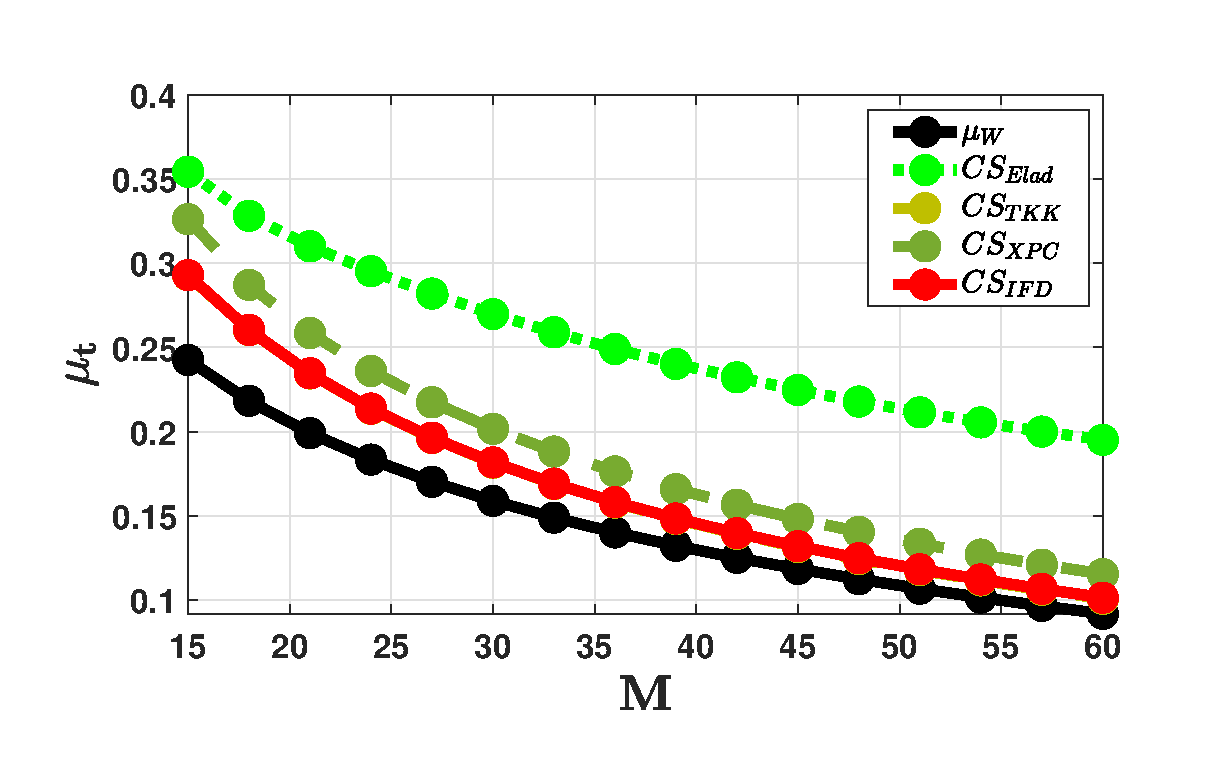
\includegraphics[keepaspectratio,width=0.47\textwidth,trim=17 10 40 25,clip]{figChap4/Mu_avg_M.eps}} 
\subfigure[Projection matrix design]{\label{fig:Mu_avg_M_projection}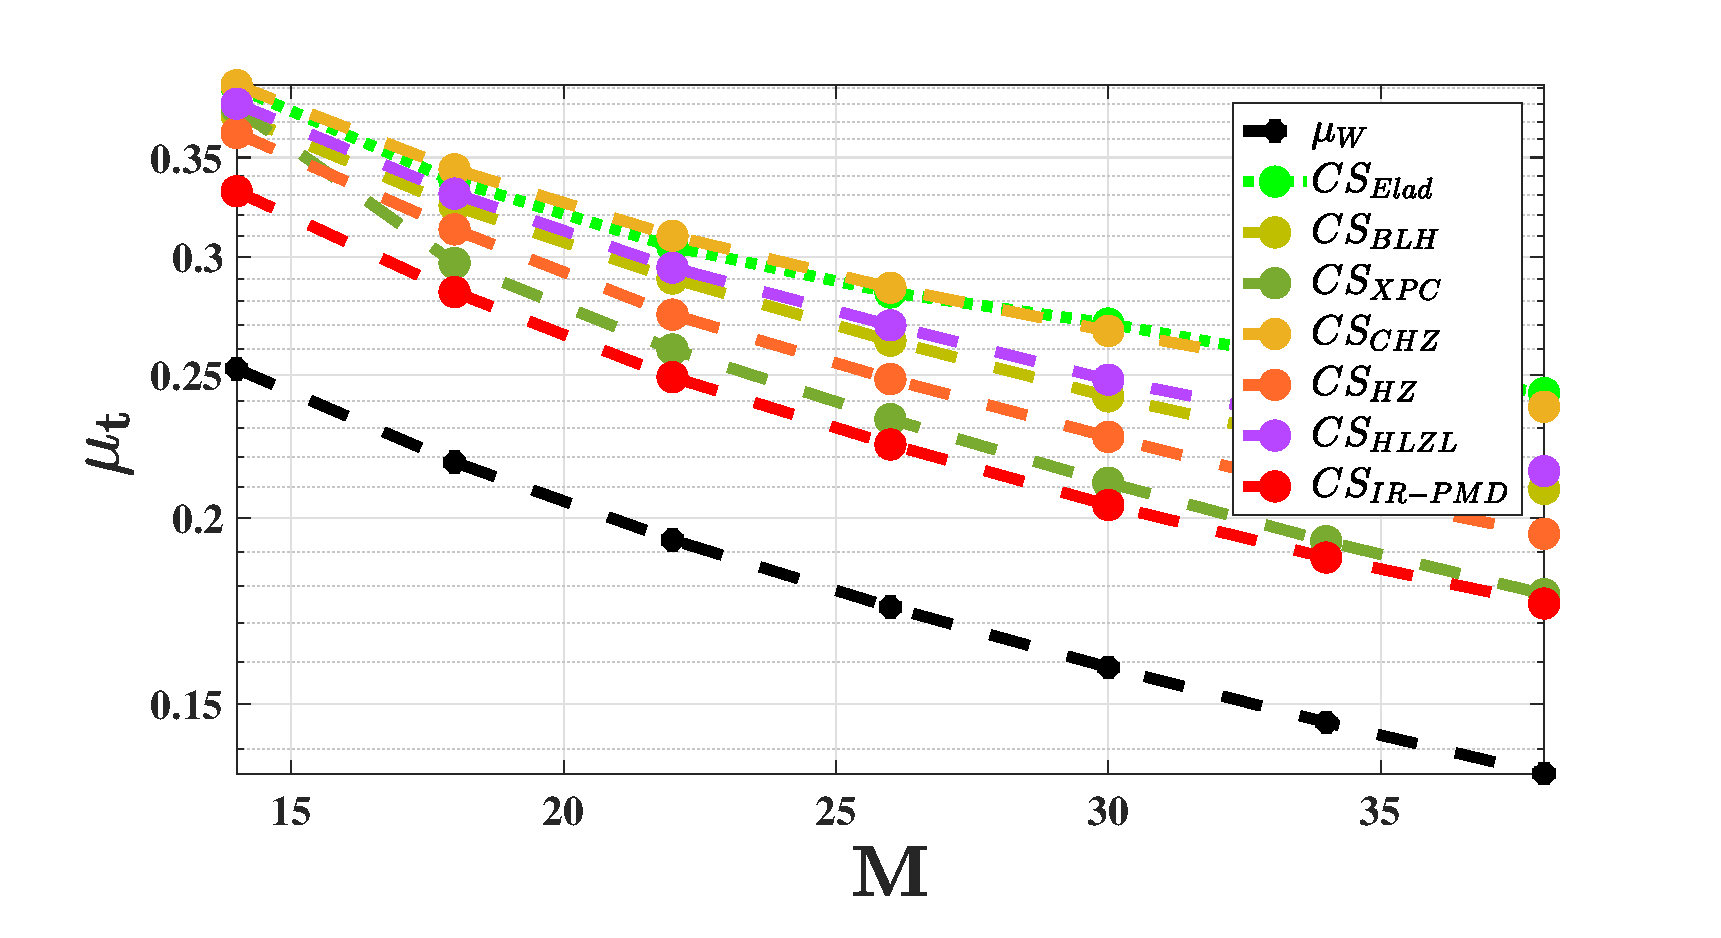
\includegraphics[keepaspectratio,width=0.52\textwidth,trim=17 10 40 25,clip]{figChap4/Muavg_M.eps}}
\caption{Averaged mutual coherence as a function of $M$ for (a) frame $\bm{D}$ and (b) projection matrix $\bm{\Phi}$ ($L=120$, SNR = $10$ dB).}
\label{Fig Coherence_M}
\end{figure}
%----------------------------------------------------%
%----------------- MU_Projection --------------------%
\begin{figure}
\centering    
\subfigure[IFD algorithm]{\label{fig: Syn_Muavg_iter}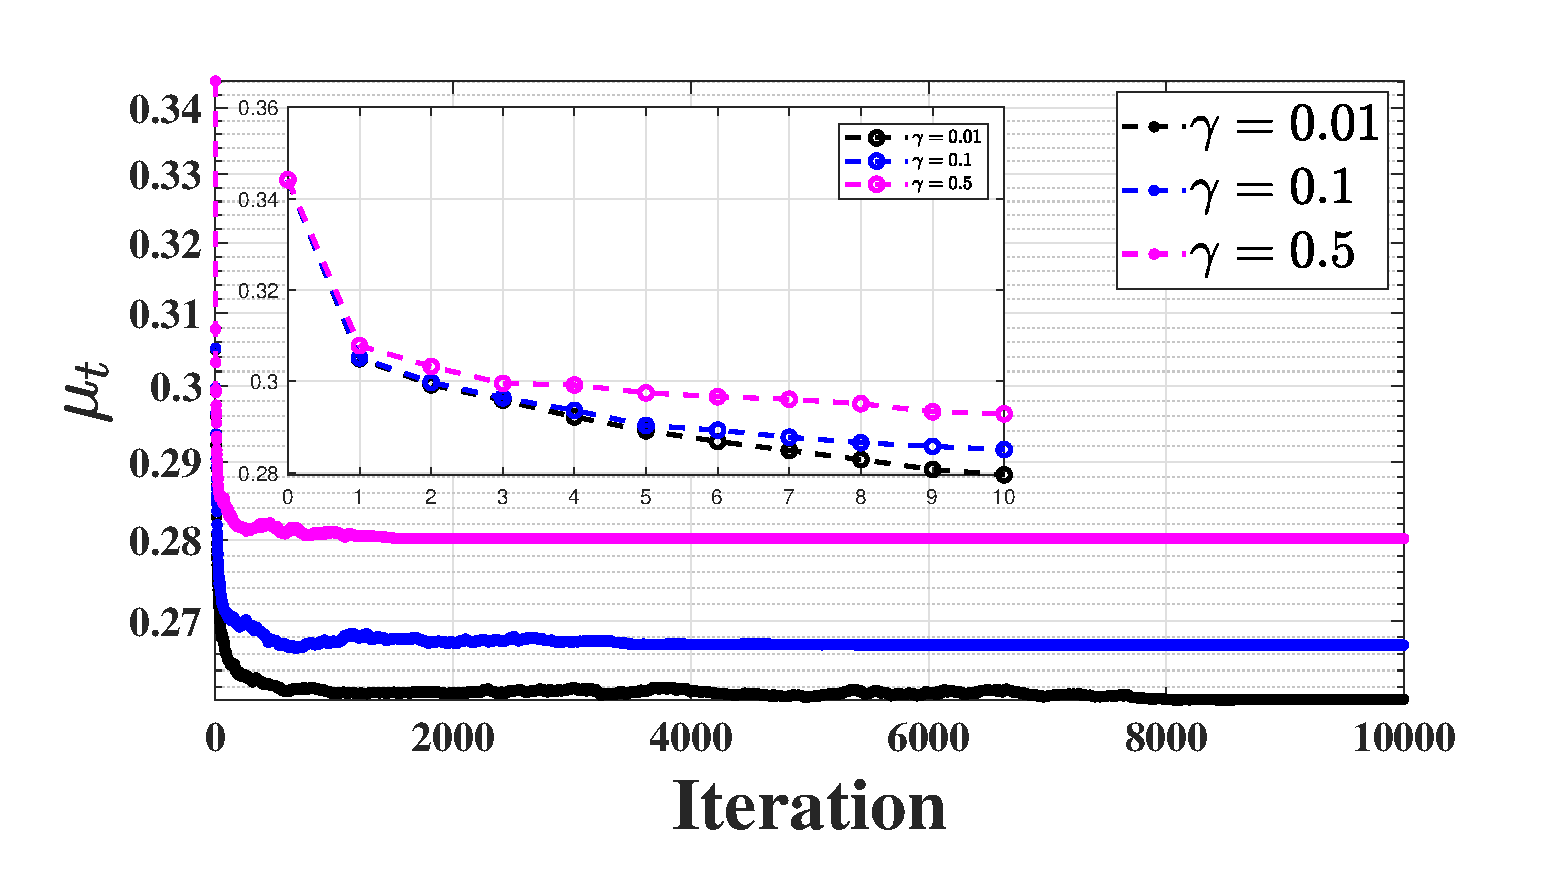
\includegraphics[keepaspectratio,width=0.47\textwidth,trim=17 10 40 25,clip]{figChap4/Muavg_Iter_at_gamma.eps}}
\subfigure[IR-PMD algorithm]{\label{fig: Cal_Muavg_iter}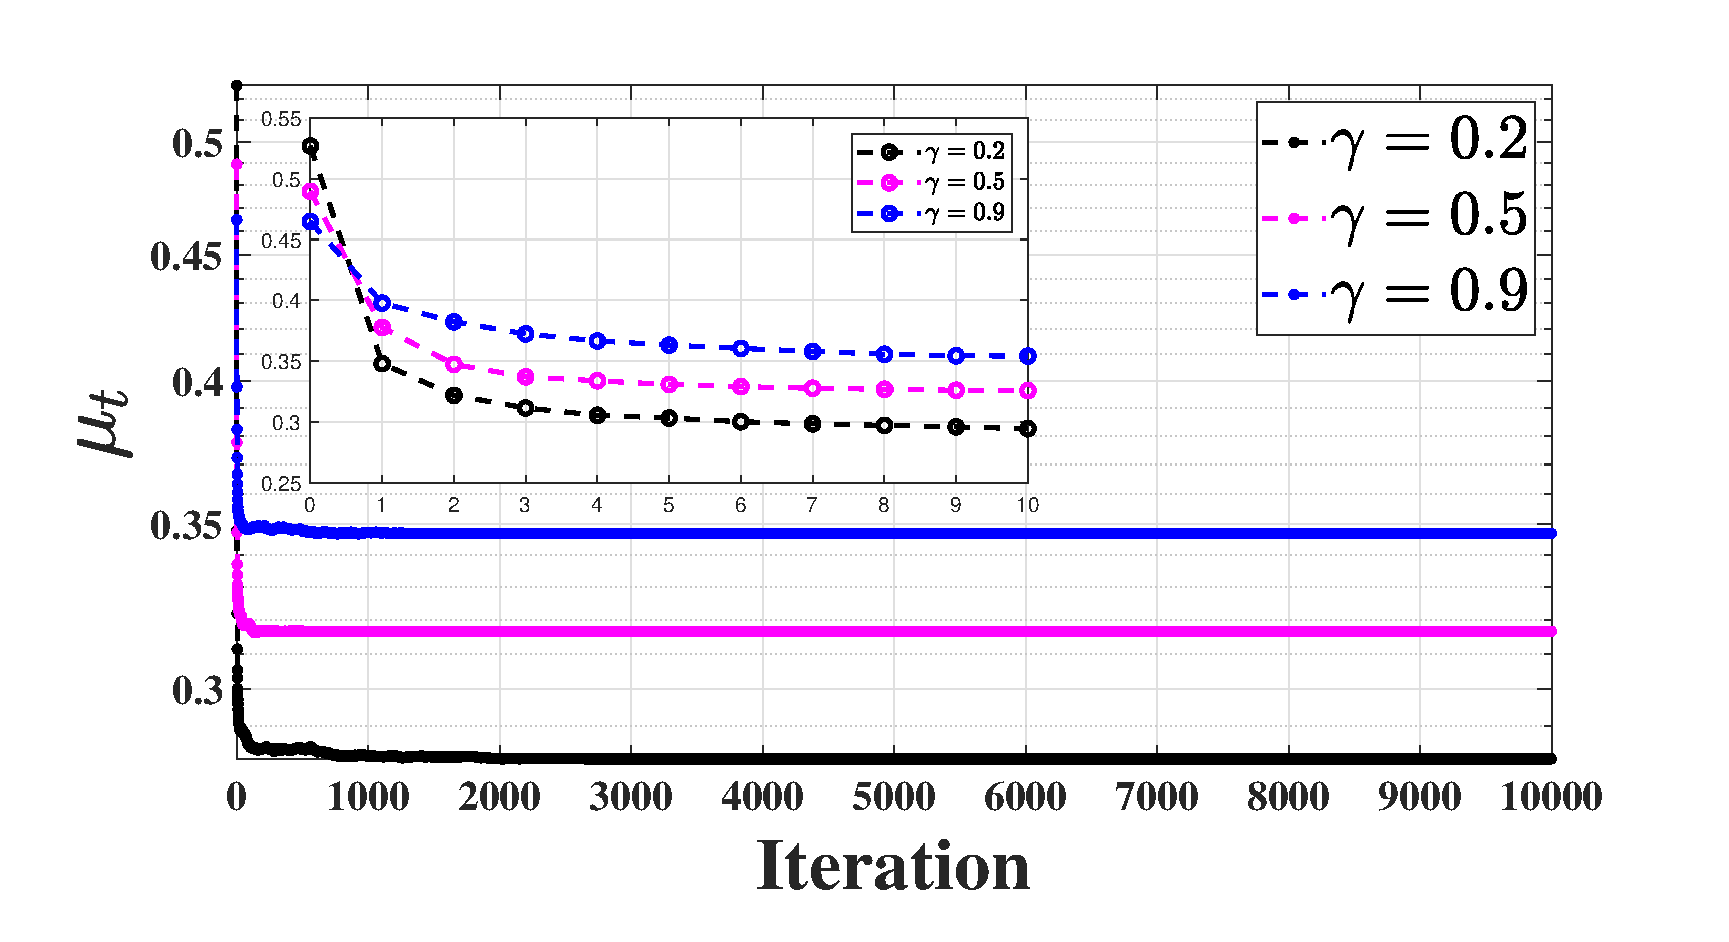
\includegraphics[keepaspectratio,width=0.47\textwidth,trim=17 10 40 25,clip]{figChap4/Cal_Muavg_iter_atgamma.eps}}
\caption{Evolution of averaged mutual coherence with the number of iterations ($L=120$, SNR = $10$ dB).}
\label{Fig Coherence_iter_at_gamma}
\end{figure}
%----------------------------------------------------%
Fig.~\ref{fig: Mu_avg_M_frame} shows the averaged mutual coherence $\mu_{t}$ (with $t=\epsilon$) for the different frame design methods as a function of the redundancy of the frame. As the number of measurements $M$ increases, all the methods achieve lower mutual coherence. The superiority of IFD algorithm is clearly evident for smaller values of $M$. The reduced mutual coherence achieved by IFD results in a tighter frame, which is then used in the IR-PMD algorithm. Similarly, for sensing matrix design approaches, Fig.~\ref{fig:Mu_avg_M_projection} shows the averaged mutual coherence $\mu_{t}$ as a function of the number of measurements. It is seen that the IR-PMD algorithm is superior compared to the other approaches. In Figs.~\ref{fig: Syn_Muavg_iter} and~\ref{fig: Cal_Muavg_iter}, evolution of the averaged mutual coherence $\mu_{t}$ is shown for different values of $\gamma$ on synthetic data sets, for IFD and IR-PMD algorithms respectively. It is seen that smaller value of $\gamma$ results in reduced mutual coherence as $\mu_{t}$ will be determined by the term $\| \overline{\bm{\Phi}}\bm{\Psi} - \overline{\bm{D}} \|_{F}^{2}$ with $\| \overline{\bm{\Phi}} \|_{F}^{2}$ being given less weight.
%%+++++++++++++++++++++++++++++++++++++++++++++++++++++++++++++%%
%-----------HISTOGRAM PROJECTION---------------------%
\begin{figure}
\centering
\hspace*{-0.5in}
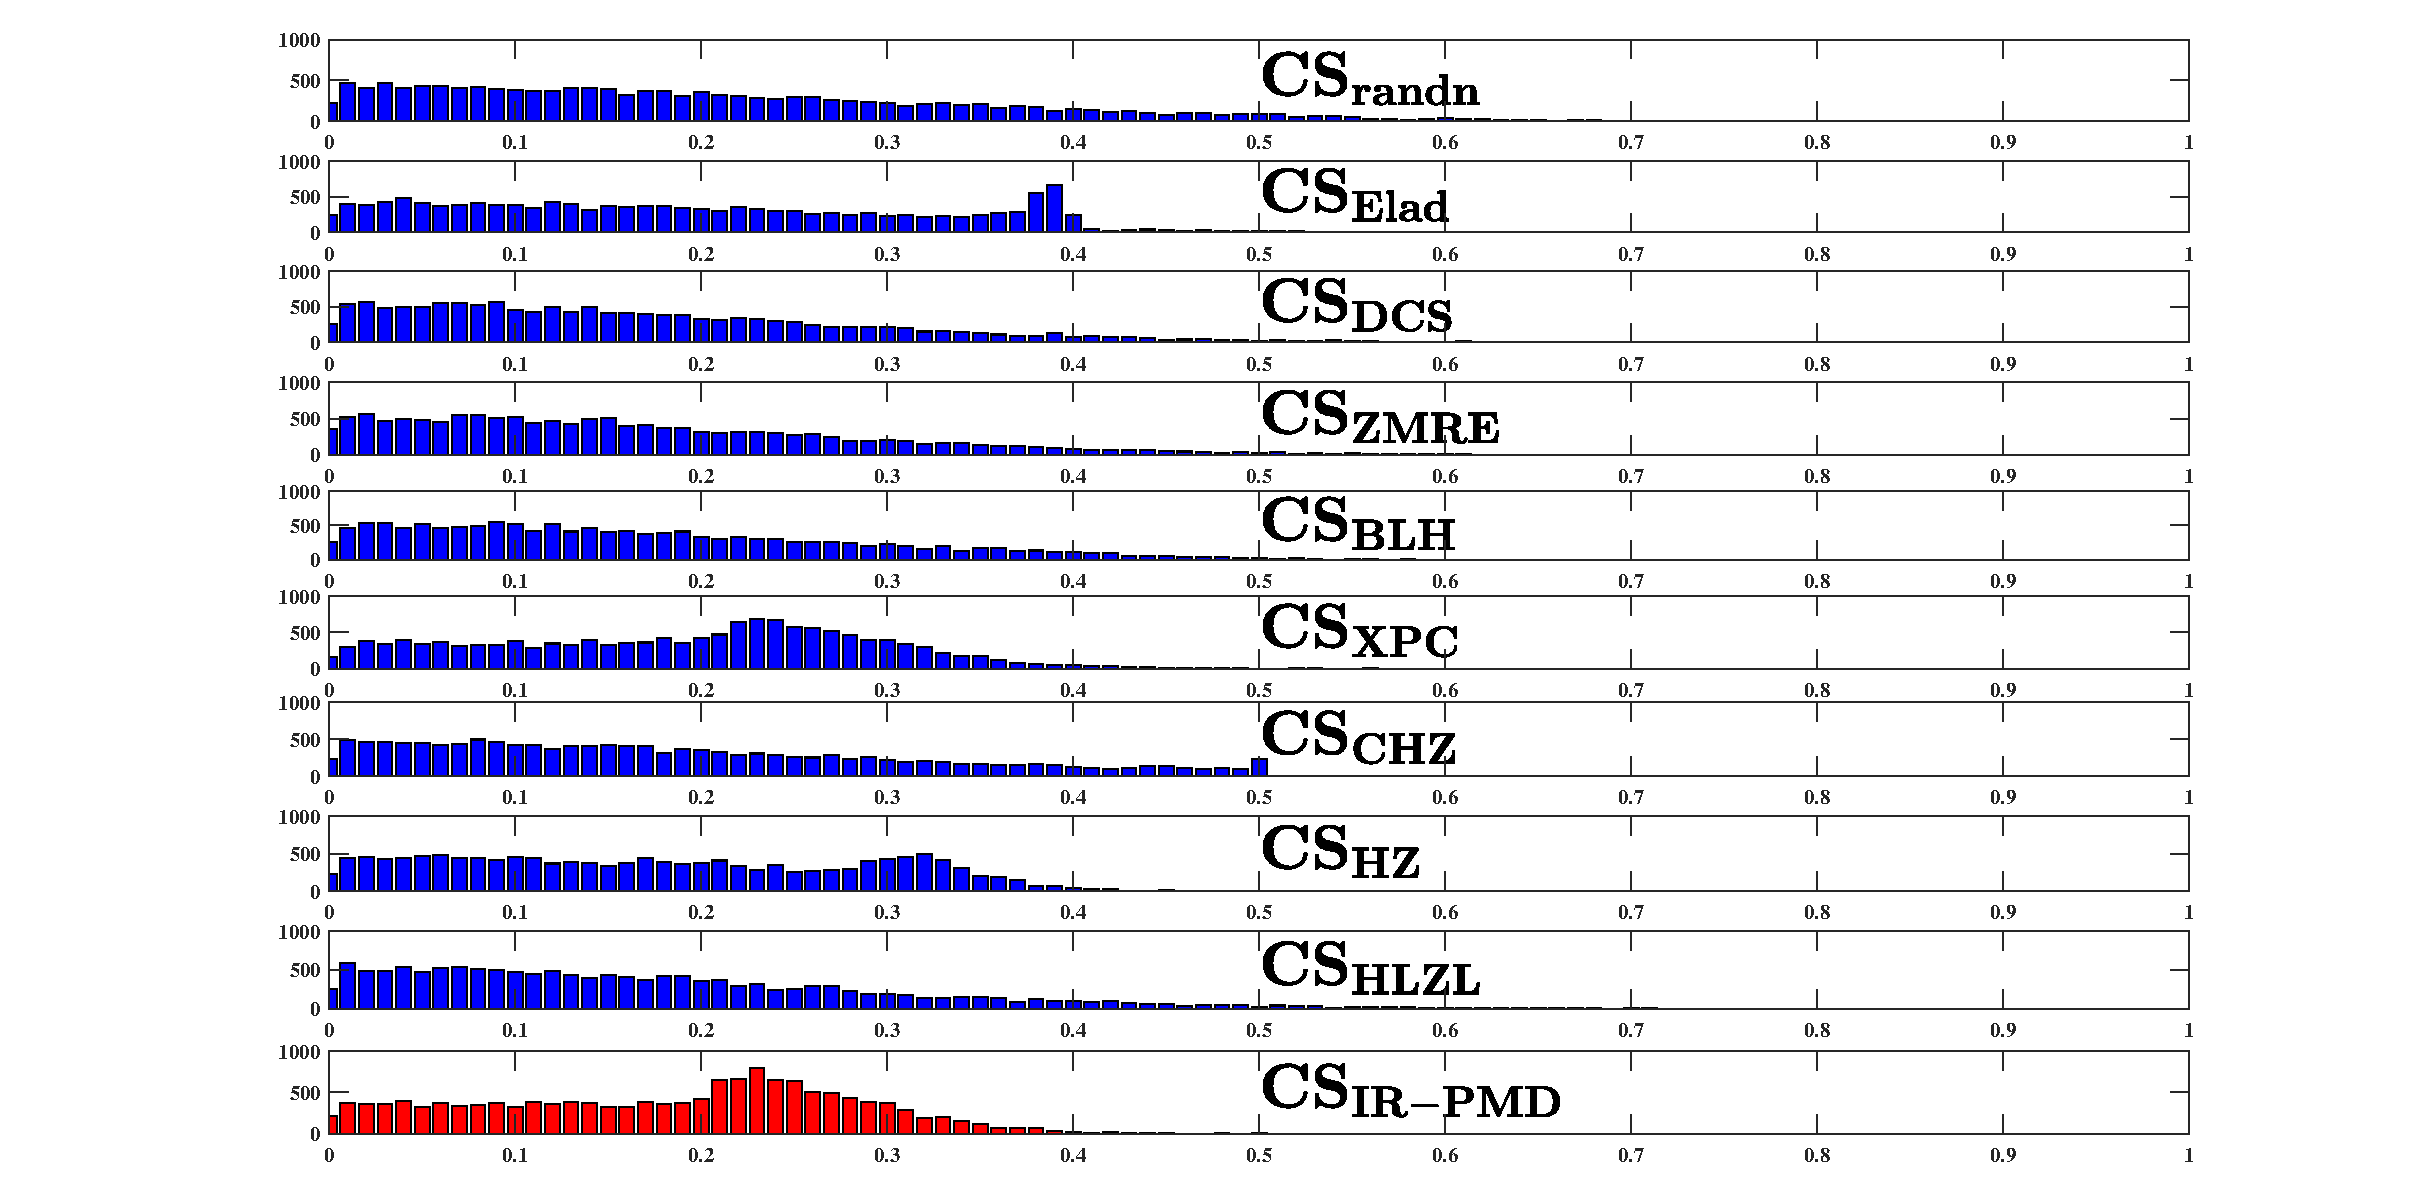
\includegraphics[keepaspectratio,width=1.1\textwidth,trim=50 20 50 20]{figChap4/Hist_10_methods.eps}
\vspace*{-0.1in}
\caption{Histogram of the absolute off-diagonal elements of the optimized Gram matrix ($N=60$, $L=120$, and $M=20$).}
\label{fig: Histogram}
\end{figure}
%--------------------------------------------------%
%%==========================================================%%
\subsubsection{Reconstruction Performance}
%
Next, we compare the different CS techniques for optimizing the sensing matrix in terms of their ability to reconstruct the original signal from under-sampled measurements. We consider a set of synthetic signals generated as earlier. The performance of the algorithms is evaluated in terms of mutual coherence and reconstruction error. The maximum number of iterations is set to $100$ for each algorithm except for the non-iterative $\text{CS}_{\text{DCS}}$~\cite{Sapiro} algorithm, and $1000$ iterations for $\text{CS}_{\text{HLZL}}$~\cite{HONG_sparse}. Each experiment is repeated $500$ times and the averaged results are presented.

For $\text{CS}_{\text{rand}}$, a normally distributed random sensing matrix is employed and this random matrix is used as the initial sensing matrix for all algorithms except $\text{CS}_{\text{ZMRE}}$ which employs the optimized matrix from $\text{CS}_{\text{DCS}}$ as the initial matrix. The parameter values for the different algorithms are selected based on the values mentioned in the corresponding references. If the optimal values were not mentioned in the references, then we carried out the parameter tuning to determine the optimal values. The MSE over a range of parameter values is computed for the methods and the parameter value resulting in minimum MSE is selected as the optimal value. The parameter values selected are as follows: (i) $\text{CS}_{\text{Elad}}$: t $=0.4$, $ \gamma=0.95$, (ii) $\text{CS}_{\text{ZMRE}}$: $\alpha=0.99$, (iii) $\text{CS}_{\text{BLH}}$: $\alpha = 0.8$~\cite{SRE_Huang}, (iv) $\text{CS}_{\text{XPC}}$: $\alpha=0.7$~\cite{Xuprojection}, (v) $\text{CS}_{\text{CHZ}}$: $\rho=0.5$, $\eta=1.2$, $\alpha=0.99\rho$, $\beta=2$, $\text{Iter}_{\text{in}}=100$ (number of inner iterations), and $\text{Iter}_{\text{out}}=15$ (number of outer iterations)~\cite{CHZ}, (vi) $\text{CS}_{\text{HZ}}$: $\lambda=0.1$ for synthetic data and $\lambda=0.9$ for real data sets~\cite{HONG_robust}, and (vii) $\text{CS}_{\text{HLZL}}$: $\lambda=0.25$, $\kappa=20$ for synthetic data and $\lambda=0.5$, $\kappa=30$ for real data sets~\cite{HONG_sparse}. Fig.~\ref{fig: Histogram} shows the histogram of the absolute off-diagonal elements of the normalized Gram matrix corresponding to the optimized sensing matrix. The proposed IR-PMD algorithm, compared to the other algorithms, results in a histogram that is centered more towards the origin which implies smaller local correlations and thus improved recovery performance. 
%
%------------------------- MU_NO -----------------------------%
\begin{table}
\caption{Coherence measures and MSE for various CS systems ($M=20$, $N=60$, $L=120$).}
\label{table: MU_MSE_NOISELESS}
\centering
\begin{tabular}{|c|c|c|c|c|}
\hline
\multirow{2}{*}{} & \multicolumn{4}{c|}{Noiseless}\\ 
\cline{2-5} 
& $\mu_{t}$ & $\mu $ & $\|\bm{I}-\bm{G}\|_{F}^{2}$ & MSE\\ 
\hline
$\text{CS}_{\text{Elad}}$~\cite{Elad} & 0.3179 & 0.7007 & 772.54 & 0.0054\\ 
\hline
$\text{CS}_{\text{DCS}}$~\cite{Sapiro} & 0.3089 & 0.6916 & 602.67 & 0.0026\\ 
\hline
$\text{CS}_{\text{ZMRE}}$~\cite{Zelnik} & 0.3088 & 0.6504 & 603.26 & 0.0029 \\ 
\hline
$\text{CS}_{\text{XPC}}$~\cite{Xuprojection} & 0.2722 & 0.5601 & 645.05 & 0.0029\\ 
\hline
$\text{CS}_{\text{CHZ}}$~\cite{CHZ} & 0.3250 & 0.5162 & 754.60 & 0.0052\\ 
\hline
$\text{CS}_{\text{BLH}}$~\cite{SRE_Huang} & 0.2651 & 0.5846 & 600.33 & 0.0031\\ 
\hline
$\text{CS}_{\text{HZ}}$~\cite{HONG_robust} & 0.2794 & \textbf{0.4275} & 612.95 & 0.0021\\ 
\hline
$\text{CS}_{\text{HLZL}}$~\cite{HONG_sparse} & 0.3104 & 0.5265 & 627.35 & 0.0037\\ 
\hline
$\text{CS}_{\text{IR-PMD}}$ & \textbf{0.2650} & 0.4663 & \textbf{600.29} & \textbf{0.0019}\\ 
\hline
\end{tabular}
\end{table}
%
%-------- NMSE_Frame 10 ------%
\begin{figure}
\centering    
\subfigure[IFD algorithm]{\label{fig: NMSE V/S K FRAME}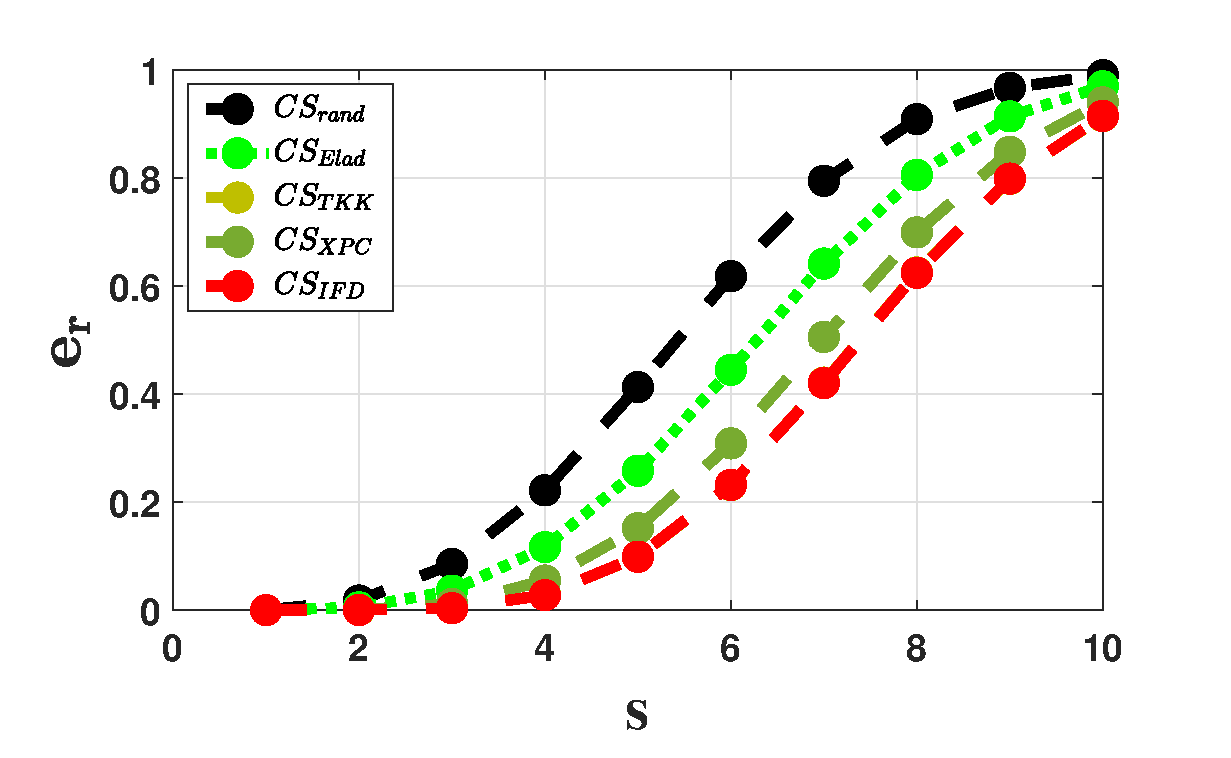
\includegraphics[keepaspectratio,width=0.47\textwidth,trim=17 0 40 25]{figChap4/NMSE_10_FRAME.eps}}
\subfigure[IR-PMD algorithm]{\label{fig: NMSE_K_PROJECTION}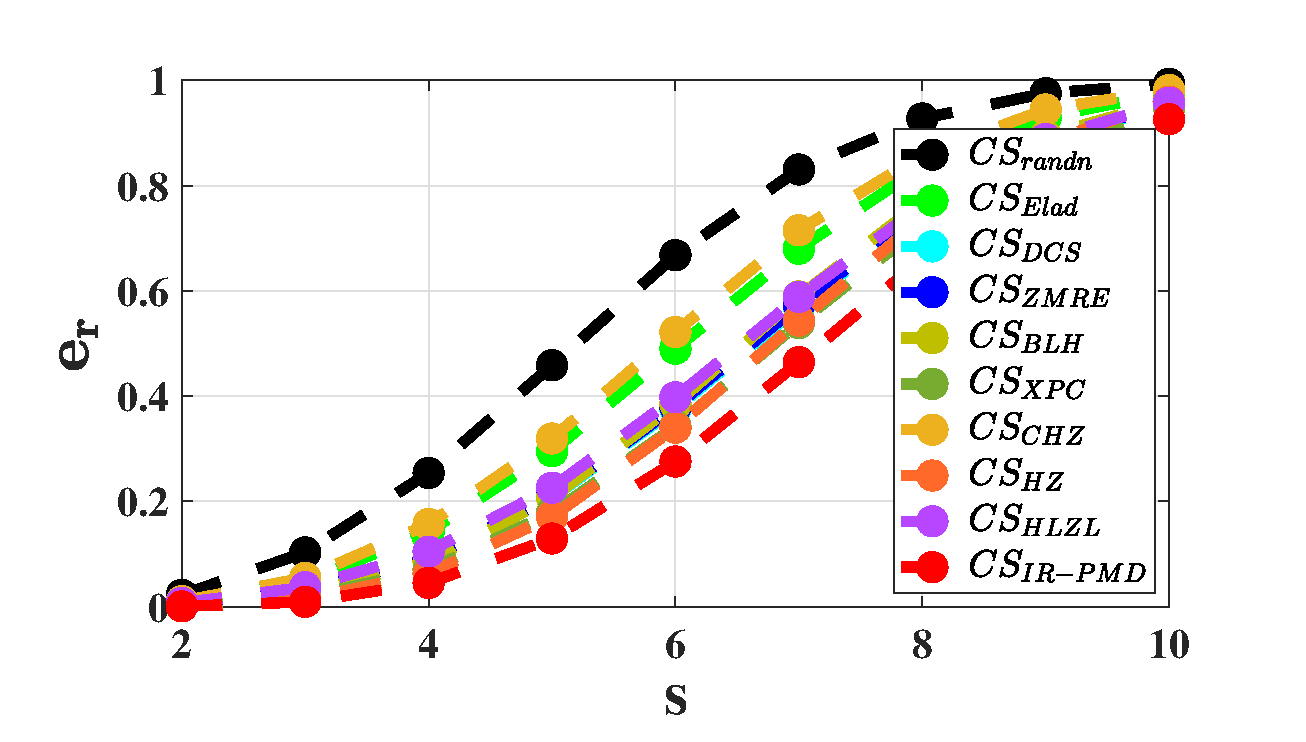
\includegraphics[keepaspectratio,width=0.52\textwidth,trim=17 0 40 25]{figChap4/Syn_NMSE_K_10.eps}}
\caption{Reconstruction error (NMSE, $e_{r}$) as a function of sparsity $s$ (SNR = $10$~dB).}
\label{Fig NMSE vs K}
\end{figure}
%-------------------------------------------------------%
%-------------------------------------------------------%
\begin{table}
\caption{Coherence measures and MSE for various CS systems ($M=20$, $N=60$, $L=120$).}
\label{table: MU_MSE_10}
\centering
\begin{tabular}{|c|cccc|}
\hline
\multirow{2}{*}{} & \multicolumn{4}{c|}{SNR = $10$ dB}\\ 
\cline{2-5} 
& \multicolumn{1}{c|}{$\mu_{t}$} & \multicolumn{1}{c|}{$\mu$} & \multicolumn{1}{c|}{$\|\bm{I}-\bm{G}\|_{F}^{2}$} & MSE\\ 
\hline
$\text{CS}_{\text{Elad}}$~\cite{Elad} & \multicolumn{1}{c|}{0.3204} & \multicolumn{1}{c|}{0.7879} & \multicolumn{1}{c|}{794.02} & 0.0042\\ 
\hline
$\text{CS}_{\text{DCS}}$~\cite{Sapiro} & \multicolumn{1}{c|}{0.3114} & \multicolumn{1}{c|}{0.6758} & \multicolumn{1}{c|}{602.75} & 0.0025\\ 
\hline
$\text{CS}_{\text{ZMRE}}$~\cite{Zelnik} & \multicolumn{1}{c|}{0.3098} & \multicolumn{1}{c|}{0.6857} & \multicolumn{1}{c|}{603.99} & 0.0028\\ 
\hline
$\text{CS}_{\text{XPC}}$~\cite{Xuprojection} & \multicolumn{1}{c|}{0.2761} & \multicolumn{1}{c|}{0.6447} & \multicolumn{1}{c|}{662.94} & 0.0026\\ 
\hline
$\text{CS}_{\text{CHZ}}$~\cite{CHZ} & \multicolumn{1}{c|}{0.3259} & \multicolumn{1}{c|}{0.5147} & \multicolumn{1}{c|}{768.65} & 0.0048\\ 
\hline
$\text{CS}_{\text{BLH}}$~\cite{SRE_Huang} & \multicolumn{1}{c|}{0.3098} & \multicolumn{1}{c|}{0.6777} & \multicolumn{1}{c|}{615.51} & 0.0025\\ 
\hline
$\text{CS}_{\text{HZ}}$~\cite{HONG_robust} & \multicolumn{1}{c|}{0.2915} & \multicolumn{1}{c|}{0.4735} & \multicolumn{1}{c|}{620.82} & 0.0028\\ 
\hline
$\text{CS}_{\text{HLZL}}$~\cite{HONG_sparse} & \multicolumn{1}{c|}{0.3133} & \multicolumn{1}{c|}{0.7285} & \multicolumn{1}{c|}{632.89} & 0.0038\\ 
\hline
$\text{CS}_{\text{IR-PMD}}$ & \multicolumn{1}{c|}{\textbf{0.2652}} & \multicolumn{1}{c|}{\textbf{0.4603}} & \multicolumn{1}{c|}{\textbf{600.25}} & \textbf{0.0015}\\ 
\hline
\end{tabular}
\end{table}
%---------------------------%
\begin{table}
\caption{MSE for various CS systems ($M=25$, $N=60$, $L=80$).}
\label{table_mse}
\centering
\begin{tabular}{|c|c|c|c|c|}
\hline
& \multicolumn{2}{c|}{Noiseless} & \multicolumn{2}{c|}{SNR = $10$ dB}\\ 
\cline{2-5}
& $s=4$ & $s=8$ & $s=4$ & $s=8$\\ 
\hline
$\text{CS}_{\text{Elad}}$~\cite{Elad} & 0.0012 & 0.0220 & 0.0013 & 0.0227\\ 
\hline
$\text{CS}_{\text{DCS}}$~\cite{Sapiro} & $2.74\mathrm{e}{-4}$ & 0.0130 & $1.87\mathrm{e}{-4}$ & 0.0142\\ 
\hline
$\text{CS}_{\text{ZMRE}}$~\cite{Zelnik} & $1.98\mathrm{e}{-4}$ & 0.0128 & $2.59\mathrm{e}{-4}$ & 0.0138\\ 
\hline
$\text{CS}_{\text{XPC}}$~\cite{Xuprojection} & $2.68\mathrm{e}{-5}$ & 0.0109 & $9.42\mathrm{e}{-5}$ & 0.0116\\ 
\hline
$\text{CS}_{\text{CHZ}}$~\cite{CHZ} & $6.44\mathrm{e}{-4}$ & 0.0211 & 0.0010 & 0.0226\\ 
\hline
$\text{CS}_{\text{BLH}}$~\cite{SRE_Huang} & $2.33\mathrm{e}{-5}$ & 0.0086 & $4.42\mathrm{e}{-4}$ & 0.0234\\ 
\hline
$\text{CS}_{\text{HZ}}$~\cite{HONG_robust} & $4.83\mathrm{e}{-6}$ & 0.0084 & $1.63\mathrm{e}{-4}$ & 0.0269\\ 
\hline
$\text{CS}_{\text{HLZL}}$~\cite{HONG_robust} & $2.77\mathrm{e}{-4}$ & 0.0124 & $2.33\mathrm{e}{-4}$ & 0.0135\\ 
\hline
$\text{CS}_{\text{IR-PMD}}$ & $\mathbf{3.33\mathrm{e}{-6}}$ & $\mathbf{0.0079}$ & $\mathbf{2.64\mathrm{e}{-5}}$ & $\mathbf{0.0081}$\\ 
\hline
\end{tabular}
\end{table}
%--------------------------------------------------%

Fig.~\ref{fig: NMSE V/S K FRAME} and Fig.~\ref{fig: NMSE_K_PROJECTION} show the NMSE ($e_{r}$) as a function of the sparsity $s$ for frame design and sensing matrix design algorithms, respectively. It is seen that the proposed IFD and IR-PMD algorithms result in reduced NMSE compared to the other algorithms. IR-PMD algorithm performs better than the mutual coherence-based methods such as $\text{CS}_{\text{Elad}}$~\cite{Elad}, $\text{CS}_{\text{DCS}}$~\cite{Sapiro}, $\text{CS}_{\text{ZMRE}}$~\cite{Zelnik}, and $\text{CS}_{\text{CHZ}}$~\cite{CHZ}. This indicates that incoherent projections are suitable for exactly sparse signals, however for signals which contain significant amount of noise it is also important to minimize the sensing matrix energy.
%------------------- vs M -------------------------%
\begin{figure}
\centering    
\subfigure[SNR = $10$~dB]{\label{fig:NMSE_M_10}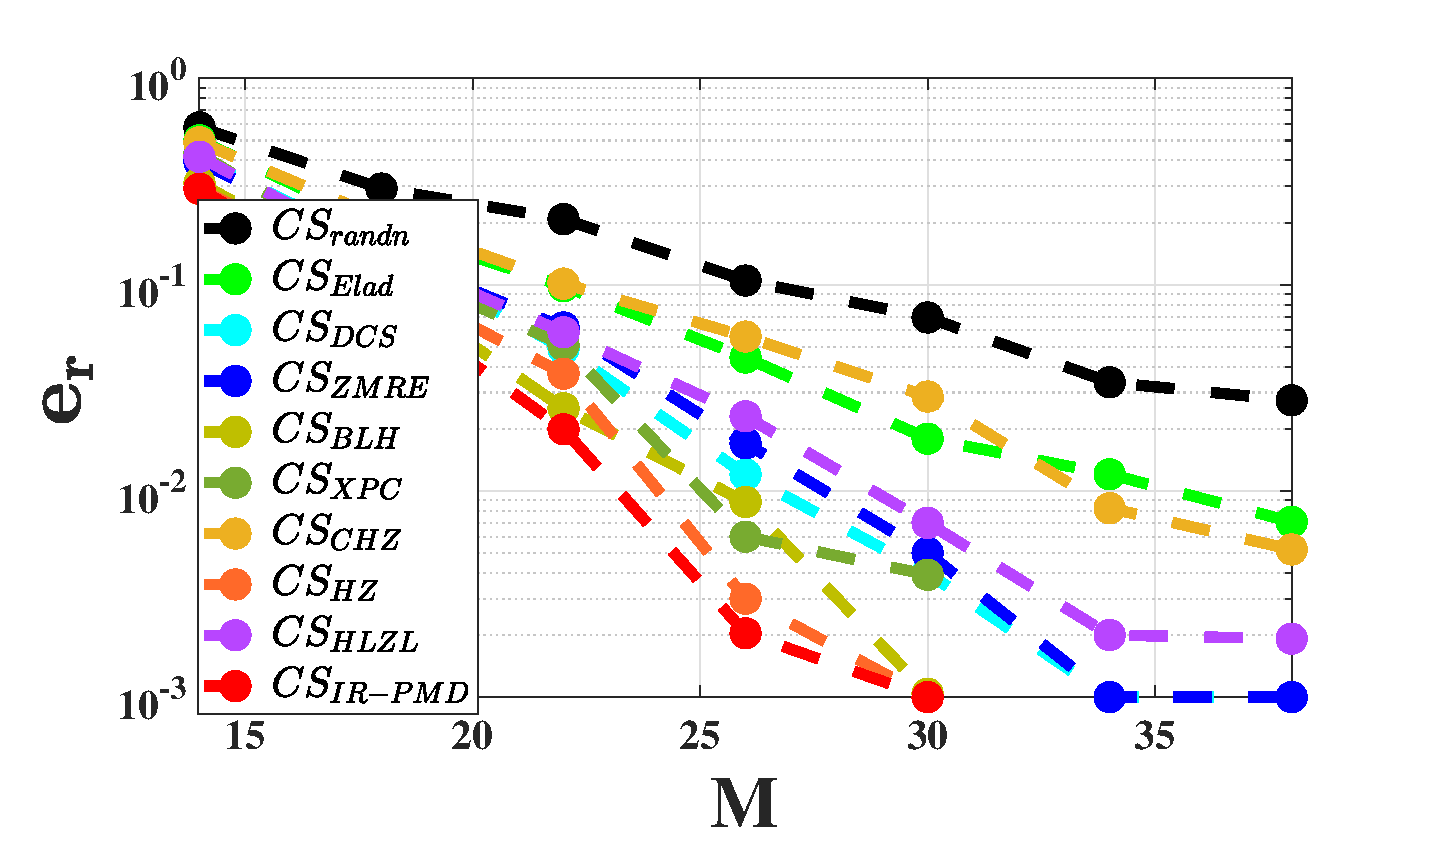
\includegraphics[keepaspectratio,width=0.44\textwidth,trim=10 5 40 5,clip]{figChap4/Syn_Nmse_M_10_new.eps}}
\subfigure[SNR = $20$~dB]{\label{fig:NMSE_M_20}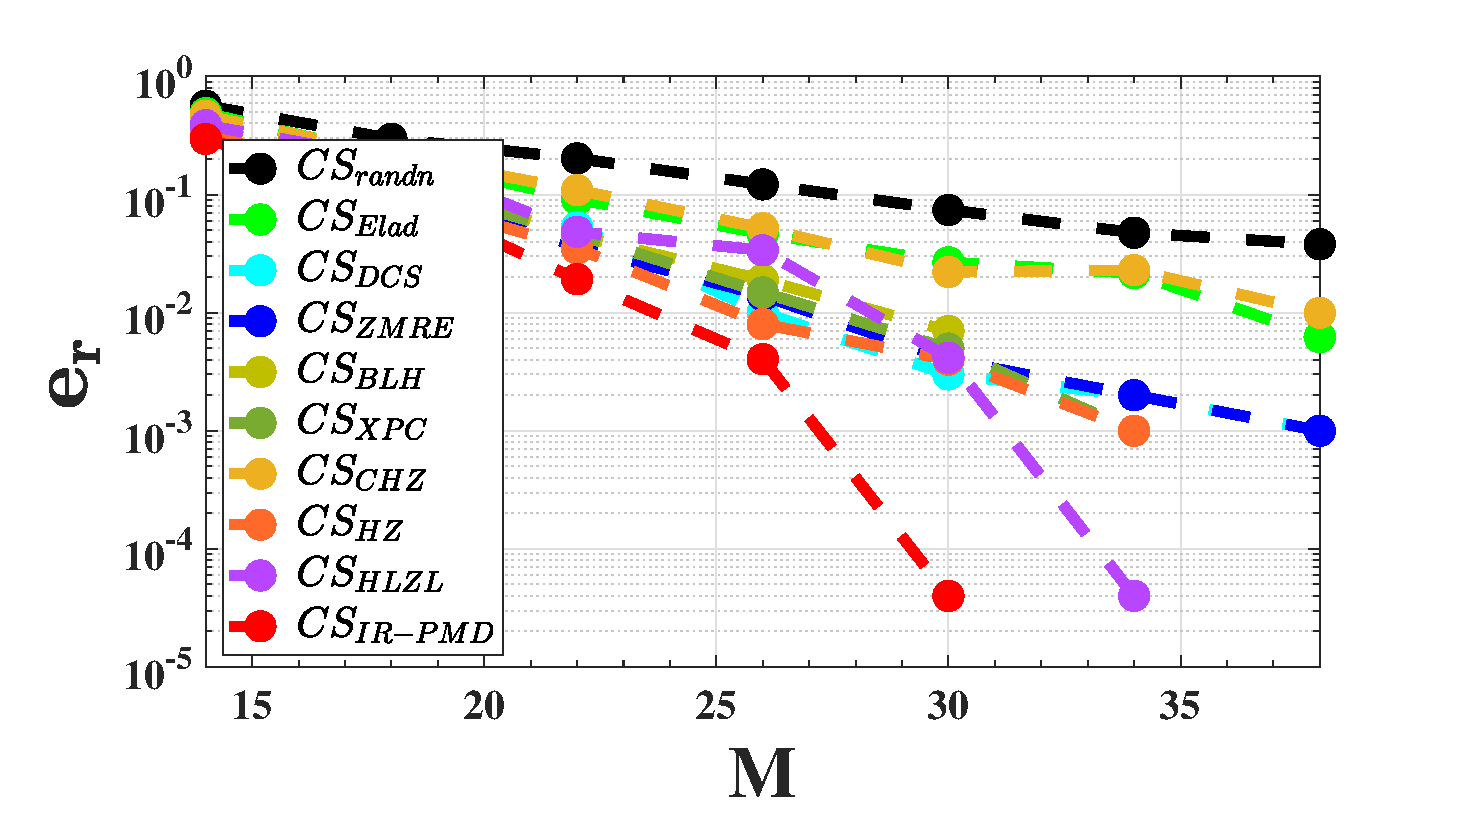
\includegraphics[keepaspectratio,width=0.46\textwidth,trim=10 5 40 5,clip]{figChap4/Syn_NMSE_M_20_new.eps}}
\caption{Recovery performance of IR-PMD model in terms of NMSE ($e_{r}$) as a function of the number of measurements $M$.}
\label{Fig NMSE V/S M PROJECTION}
\end{figure}

In Tables~\ref{table: MU_MSE_NOISELESS} and~\ref{table: MU_MSE_10}, for each CS technique, we study the performance of the optimized sensing matrix in terms of $\mu$, $\mu_{t}$, $\|\bm{I}-\bm{G}\|_{F}^{2}$, and MSE under noiseless and noisy scenarios. For the noiseless case, sensing matrix with reduced mutual coherence leads to improved signal reconstruction, however this is not true for the noisy scenario. Even though mutual coherence using IR-PMD algorithm is not significantly reduced, use of the $\ell_{2,1}$-norm results in improved signal reconstruction at low SNRs as shown in Table~\ref{table_mse}. The improved MSE is due to robustness of the $\ell_{2,1}$-norm to outliers. However, for the noiseless case, $\text{CS}_\text{BLH}$ has reduced MSE than IR-PMD due to the Frobenius norm used to minimize the mutual correlation. This shows that mutual coherence is not the best measure for estimating signal recovery performance when the signals contain significant amount of noise. For achieving a robust CS system, we consider the encoding error in order to reduce the effect of noise on the signal recovery process.

In Fig.~\ref{Fig NMSE V/S M PROJECTION}, we study the recovery performance of CS systems as a function of the number of measurements $M$ with $s=4$, and for two different SNRs. Figs.~\ref{fig: NMSE_K_PROJECTION} and~\ref{Fig NMSE V/S M PROJECTION} clearly demonstrate the superior recovery performance of the proposed IR-PMD algorithm. In Fig.~\ref{Fig NMSE V/S L PROJECTION}, we show the recovery performance as a function of the number of dictionary atoms $L$. For higher SNRs, the performance of the mutual coherence based methods and the proposed algorithm are comparable. The $\ell_{2,1}$-norm based IR-PMD algorithm is found to be more robust against the encoding error and therefore is well suited for applications such as image compression where the sparse encoding error is significant.
%------- NMSE v/s L -------------%
\begin{figure}
\centering    
\subfigure[SNR = $10$~dB]{\label{fig:NMSE_L_10}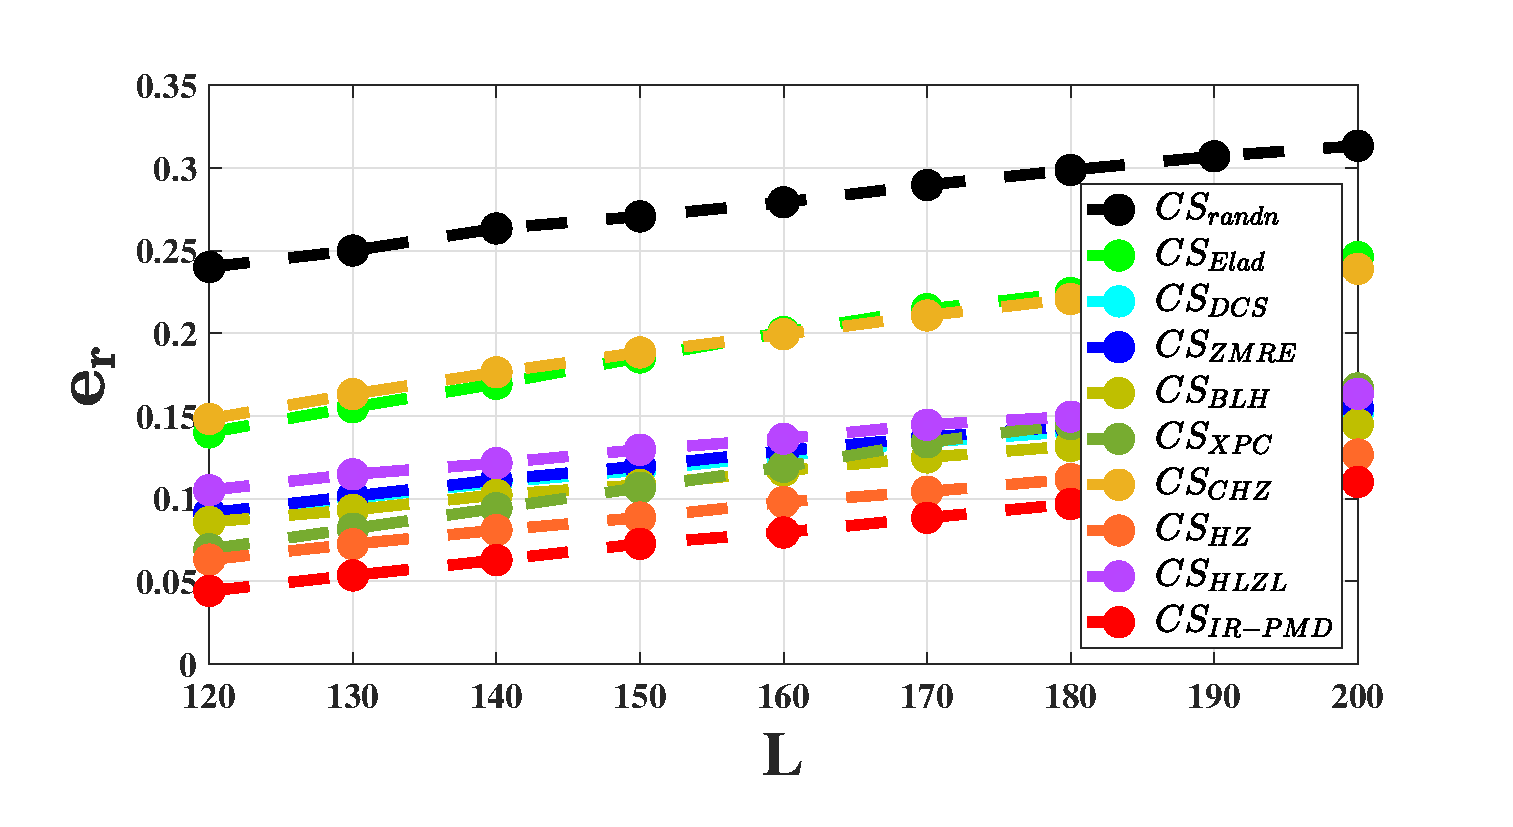
\includegraphics[keepaspectratio,width=0.47\textwidth,trim=17 10 40 25,clip]{figChap4/Syn_Nmse_L_10.eps}}
\subfigure[SNR = $20$~dB]{\label{fig:NMSE_L_20}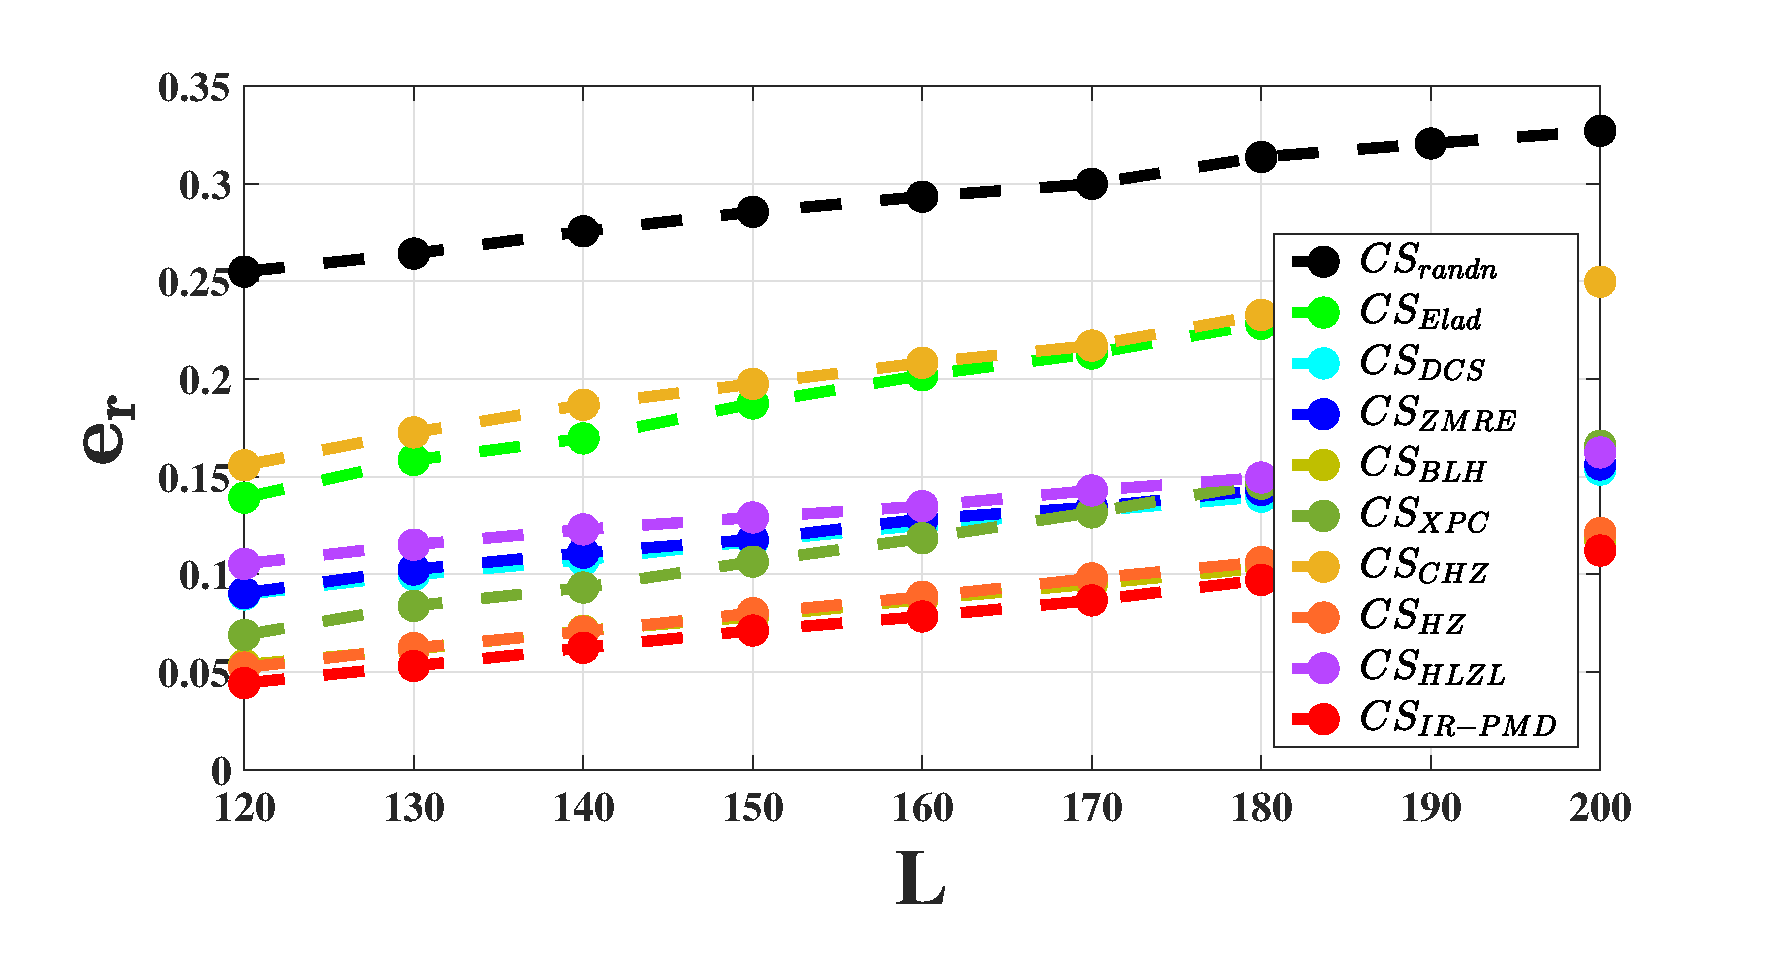
\includegraphics[keepaspectratio,width=0.47\textwidth,trim=17 10 40 25,clip]{figChap4/Syn_NMSE_L_20.eps}} 
\caption{Recovery performance error NMSE ($e_{r}$) as a function of the number of dictionary atoms $L$.}
\label{Fig NMSE V/S L PROJECTION}
\end{figure}
%---- Results for Real Data --------%
%-----------------------------------%
%
%\subsection{Optimized Projections for Image Compression}
%
\subsection{Performance Evaluation on Real Data}
%
To demonstrate the practical applicability of the proposed method we perform experiments on standard real images. We investigate the applicability of the proposed CS system for image compression. The objective is to recover the original images from their compressed versions via optimized projections. For sparse representation of the images, we learn the transform basis $\bm{\Psi}$ using KSVD~\cite{KSVD}. It is difficult to learn the ground truth dictionary for a set of real images and there will always be a non-zero encoding error even without any additional noise. Similar to the experiments with synthetic data, we set the parameters as $s=4$, $M=20$, and $L=100$. We evaluate the recovery performance of the proposed method via two experiments involving standard images and Caltech-101 data set~\cite{Caltech101}.
%
\subsubsection{Standard Images}
\label{subsec: Chap4_standard}
%
In this experiment, we use a collection of $40$ well-known standard images, including Cameraman, Elaine, Lena, and Pirate. From these images, we obtain $60,000$ patches each of size $8 \times 8$ pixels. Of these $50,000$ patches are used for training and the remaining $10,000$ are used for testing the recovery performance of the optimized projections and its generalization capability. Each patch is represented as a $64 \times 1$ vector with the set of patches expressed as a matrix of size $64 \times 60000$. We evaluate the recovery performance on the test data by adding white Gaussian noise with the resulting SNR ranging from $5$ dB to $45$ dB. The recovery performance for image compression is typically measured in terms of the PSNR given in~\eqref{eq: PSNR} and MSE given in~\eqref{eq: MSE_error}. The averaged MSE performance of different CS systems over $1000$ trials is shown in Fig.~\ref{fig: MSE_SNR_real}. It is seen that at low SNRs even random projections perform better than some of the mutual coherence-based approaches. The proposed IR-PMD algorithm has improved performance and is able to reduce the effect of noise. Fig.~\ref{fig: PSNR_SNR_real} shows the PSNR performance as a function of the SNR. Note that IR-PMD performs better than the approaches in~\cite{HONG_robust, HONG_sparse, SRE_Huang} which shows the impact of the $\ell_{2,1}$-norm and adaptive weight penalty in achieving improved robustness.
%
%-------------------- PSNR MSE_snr_Diff --------------------------%
\begin{figure}
\centering    
\subfigure[MSE versus SNR]{\label{fig: MSE_SNR_real}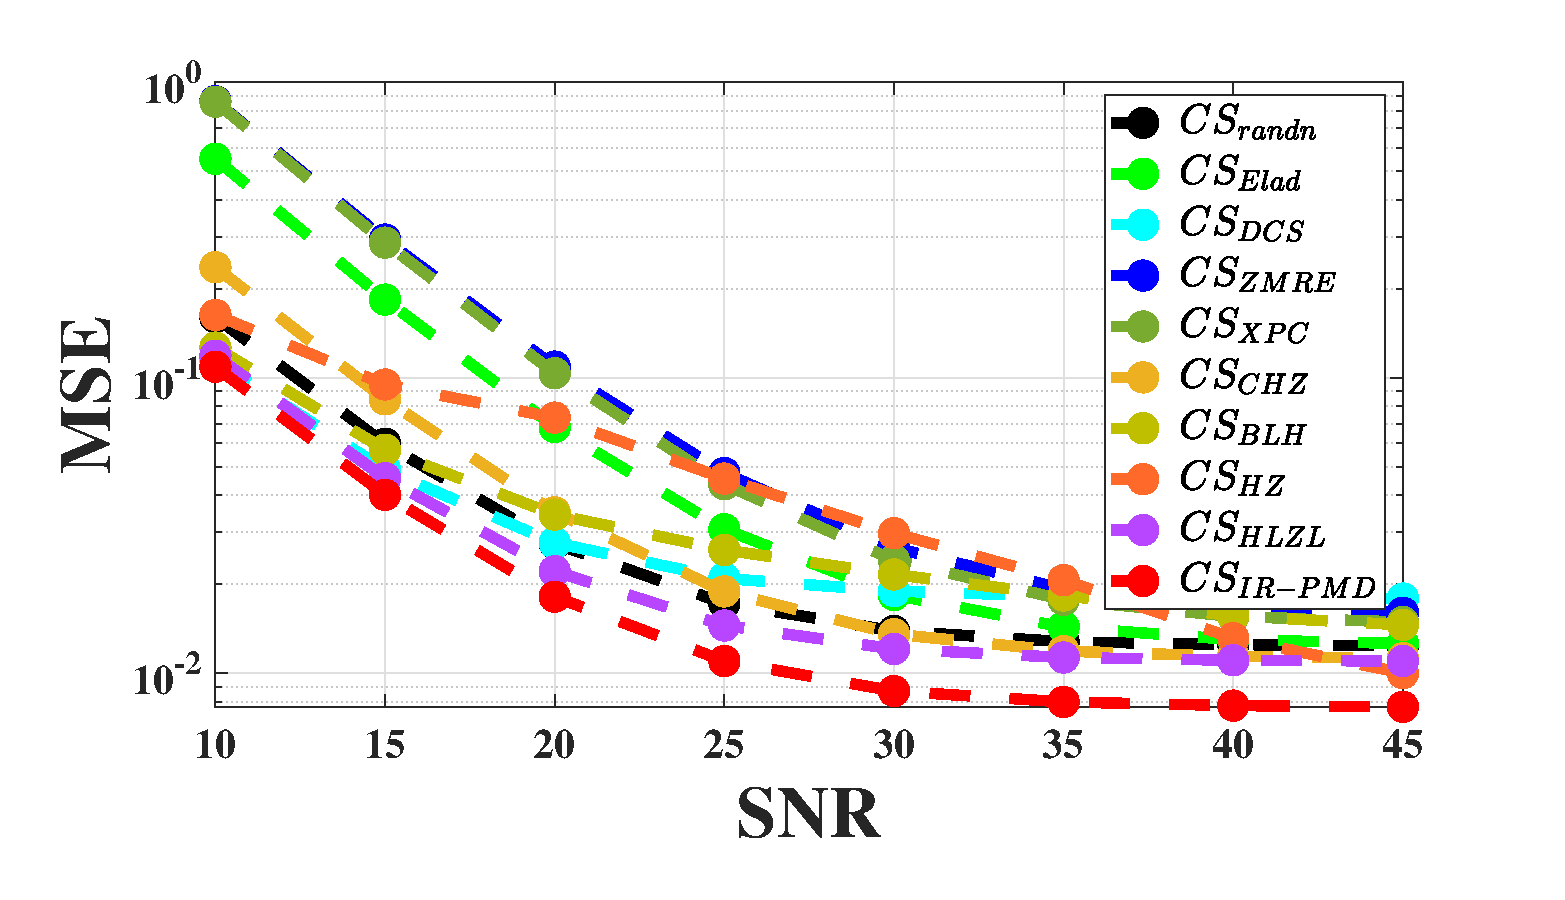
\includegraphics[keepaspectratio,width=0.48\textwidth,trim=5 5 40 5,clip]{figChap4/STD_MSE_SNR.eps}}
\subfigure[PSNR versus SNR]{\label{fig: PSNR_SNR_real}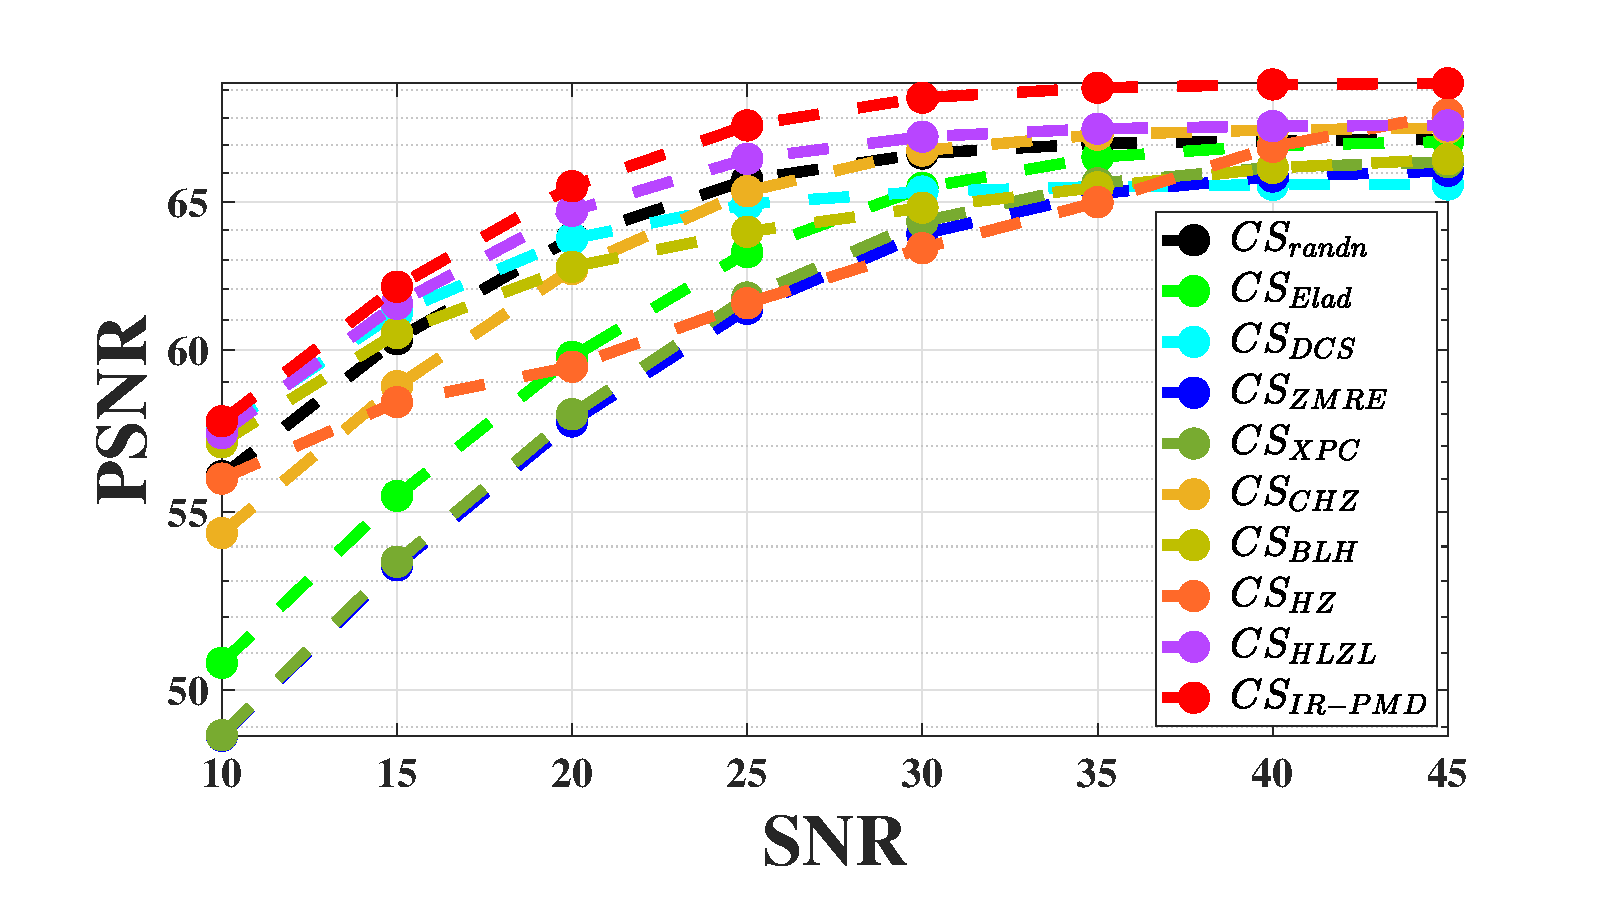
\includegraphics[keepaspectratio,width=0.49\textwidth,trim=5 5 40 5,clip]{figChap4/STD_PSNR_SNR.eps}}
\caption{MSE and PSNR as a function of SNR for optimized projections ($N=64$, $L=100$, and $M=20$).}
\label{Fig MSE PSNR V/S SNR}
\end{figure}
%
%----------- PSNR V/S SNR Dataset 2------------------%
\begin{figure}
\centering    
\subfigure[MSE versus SNR]{\label{fig: NMSE_SNR_label}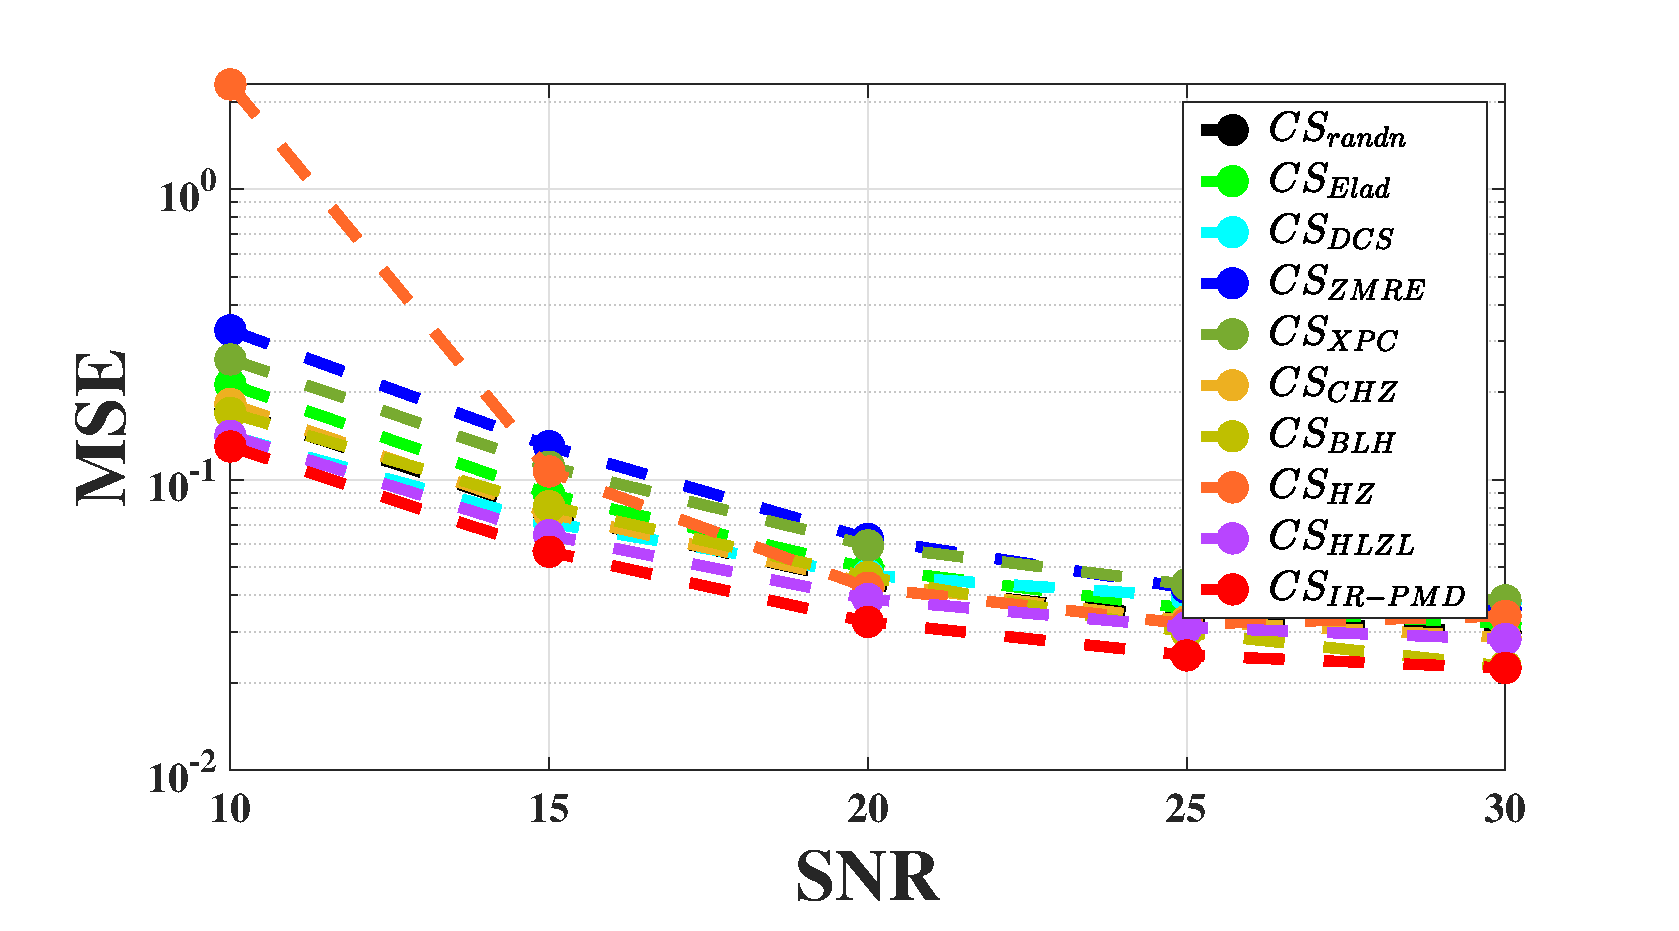
\includegraphics[keepaspectratio,width=0.49\textwidth,trim=5 5 40 5,clip]{figChap4/Caltech_MSE_snr.eps}}
\subfigure[PSNR versus SNR]{\label{fig: PSNR_SNR_label}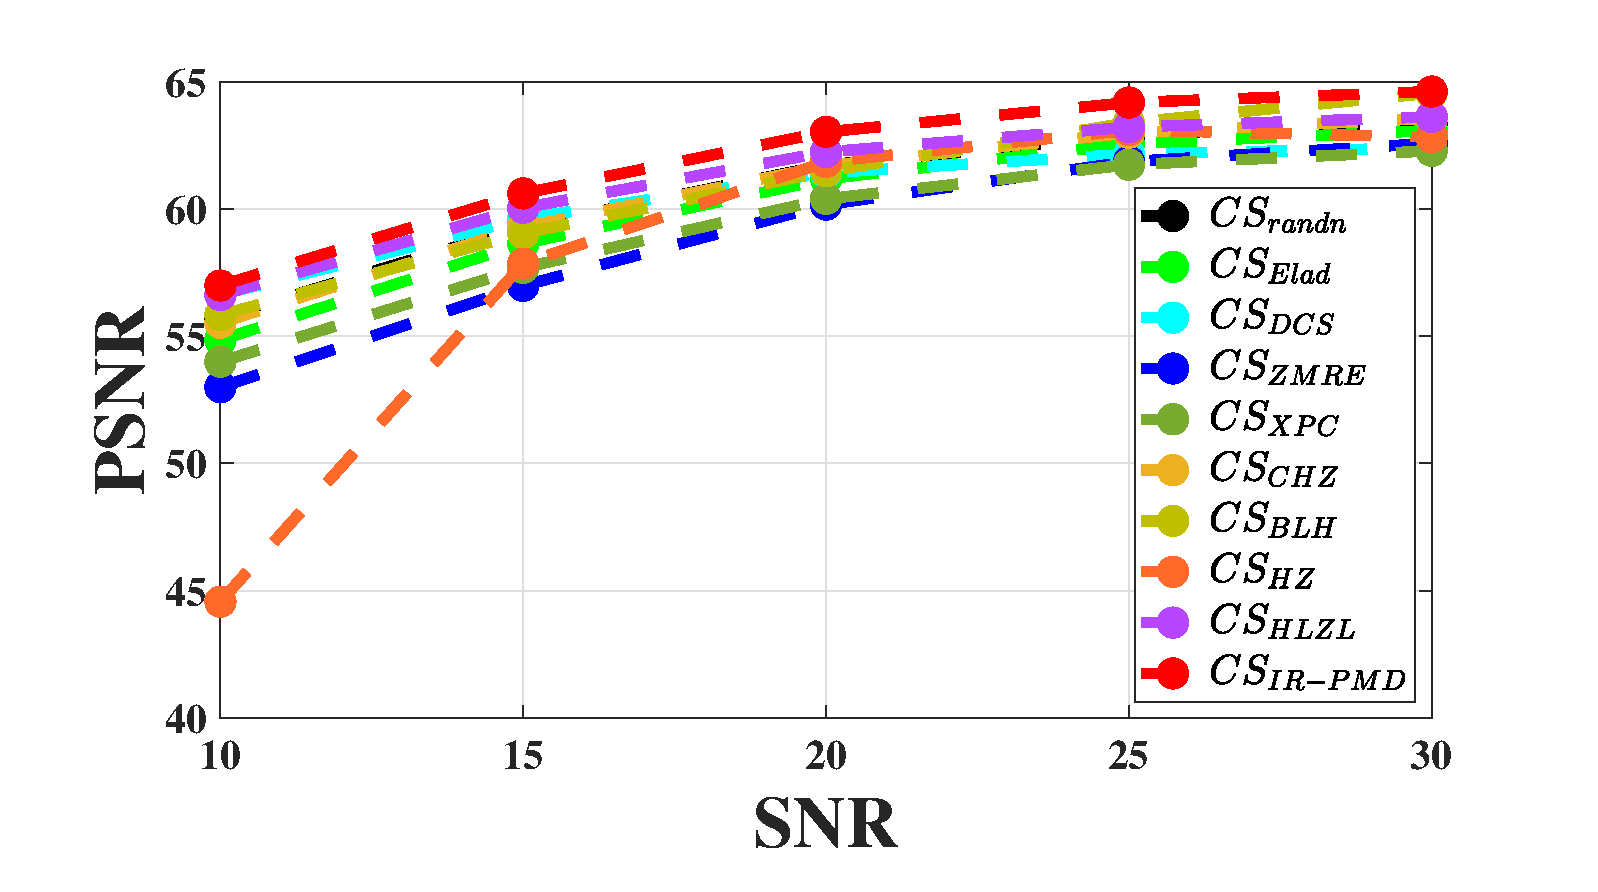
\includegraphics[keepaspectratio,width=0.49\textwidth,trim=5 5 40 5,clip]{figChap4/Caltech_PSNR_snr.eps}}
\caption{MSE and PSNR as a function of SNR for optimized projections ($N=64$, $L=100$, and $M=20$) using Caltech 101 data set.}
\label{Fig CAL MSE PSNR v/s SNR}
\end{figure}
%--------------------------------------------------%
%--------------------------------------------------%
\begin{figure}
\centering
  \begin{tabular}{@{}ccc@{}}
   \subfigure[Original image:~\textit{Cameraman}]{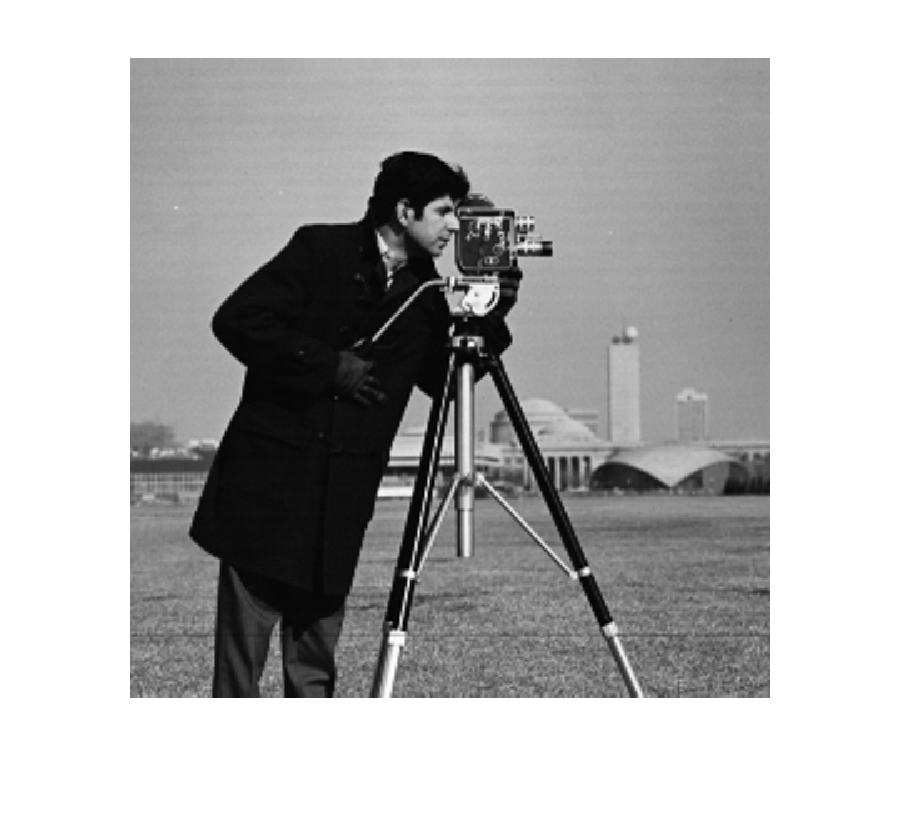
\includegraphics[width=.30\textwidth]{figChap4/cameraman_orig.eps}} &
    \subfigure[Original image:~\textit{Pirate}]{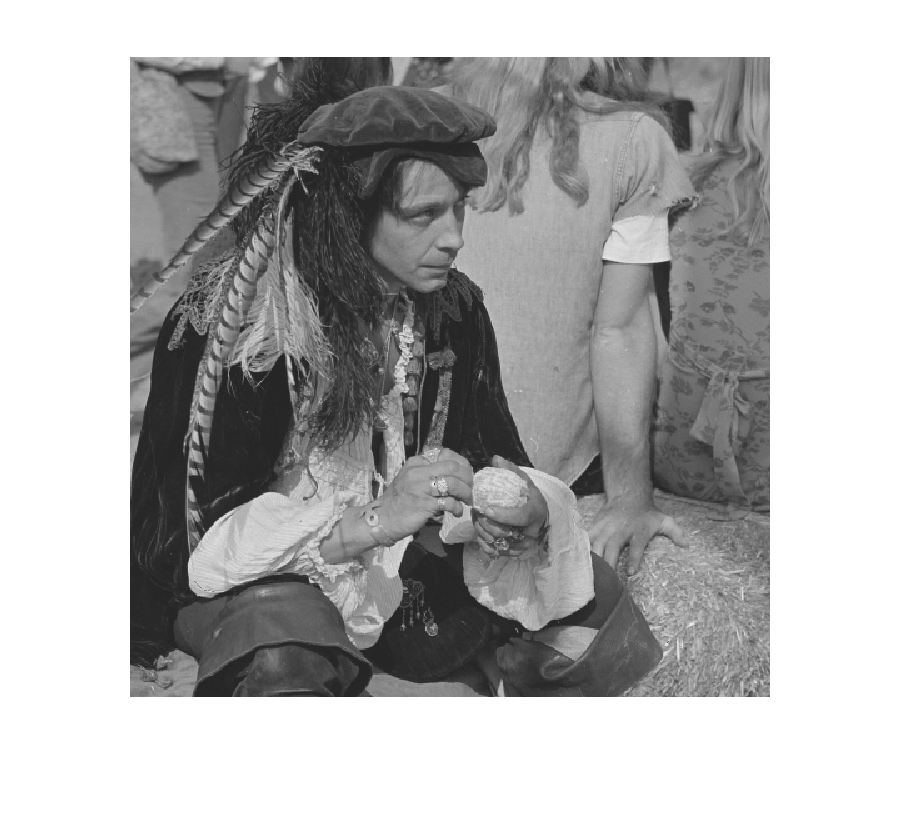
\includegraphics[width=.30\textwidth]{figChap4/pirate_orig.eps}}&
    \subfigure[Original image:~\textit{Elaine}]{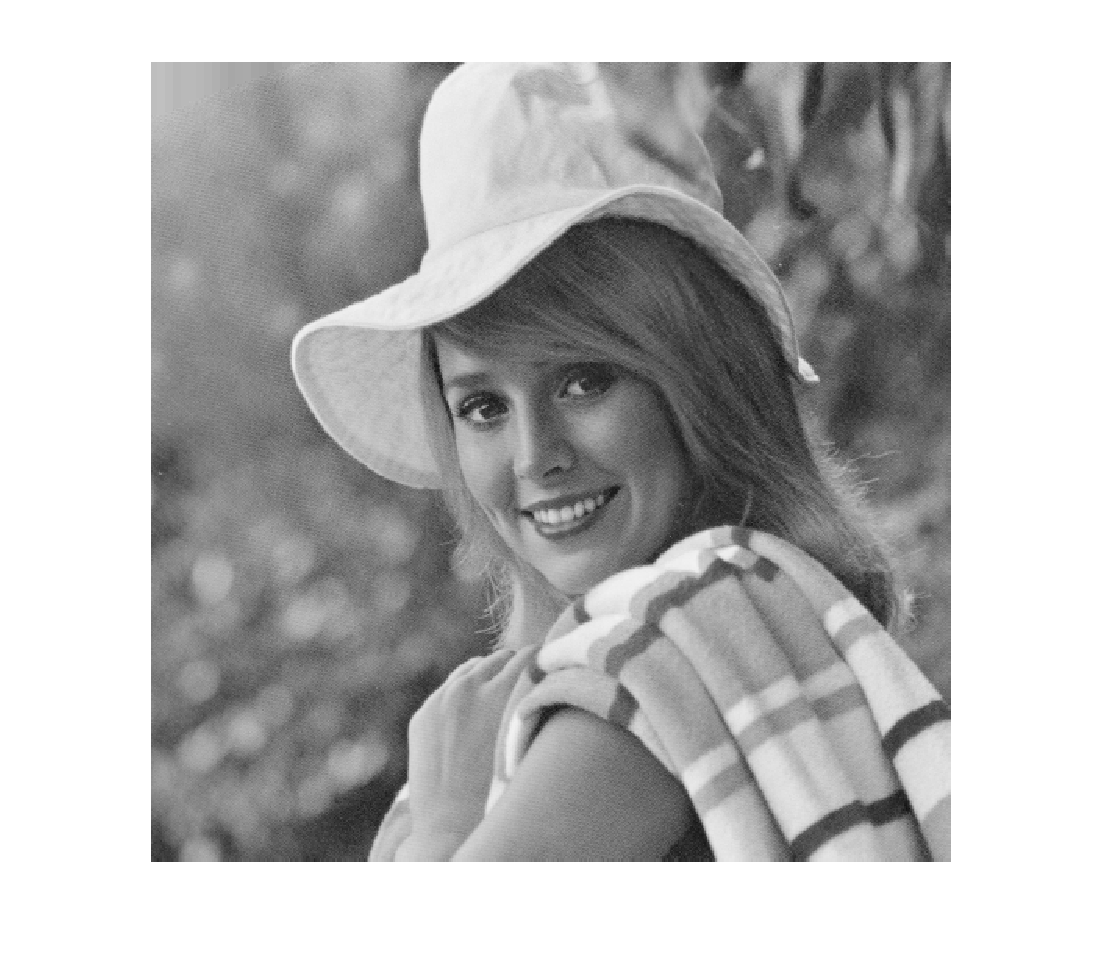
\includegraphics[width=.30\textwidth]{figChap4/Elaine_org.eps}}\\
    \subfigure[$\text{CS}_{\text{HLZL}}$ with PSNR = $32.52$~dB]{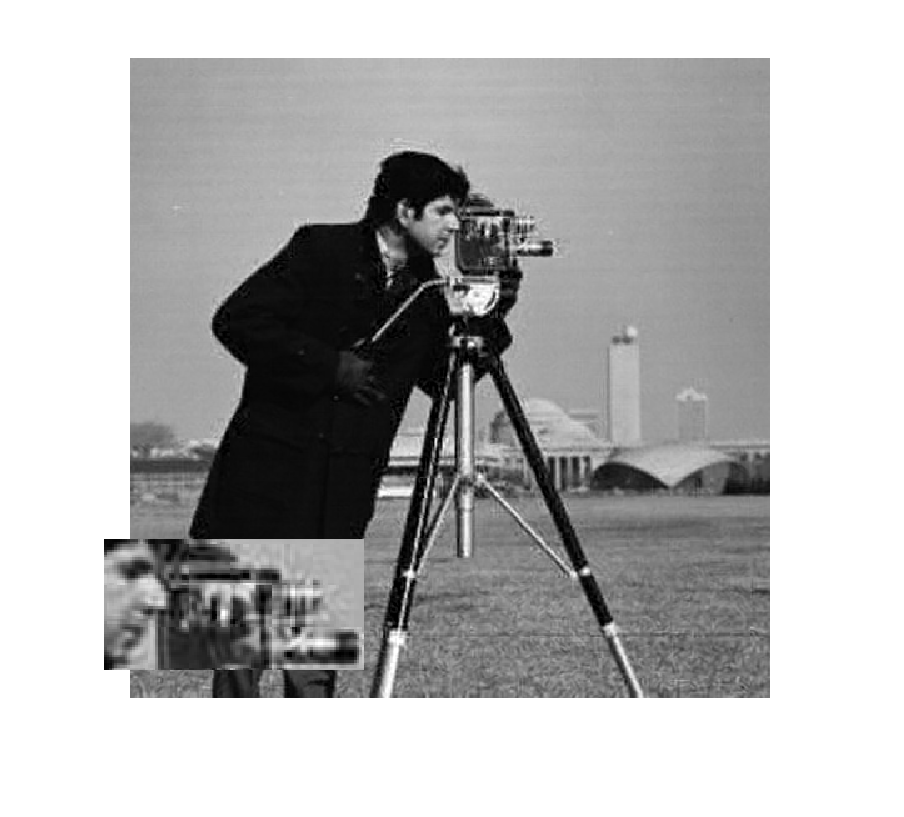
\includegraphics[width=.30\textwidth]{figChap4/Fig_Cam_hlzl_camface_zoom.eps}} &
    \subfigure[$\text{CS}_{\text{HLZL}}$ with PSNR = $29.09$~dB]{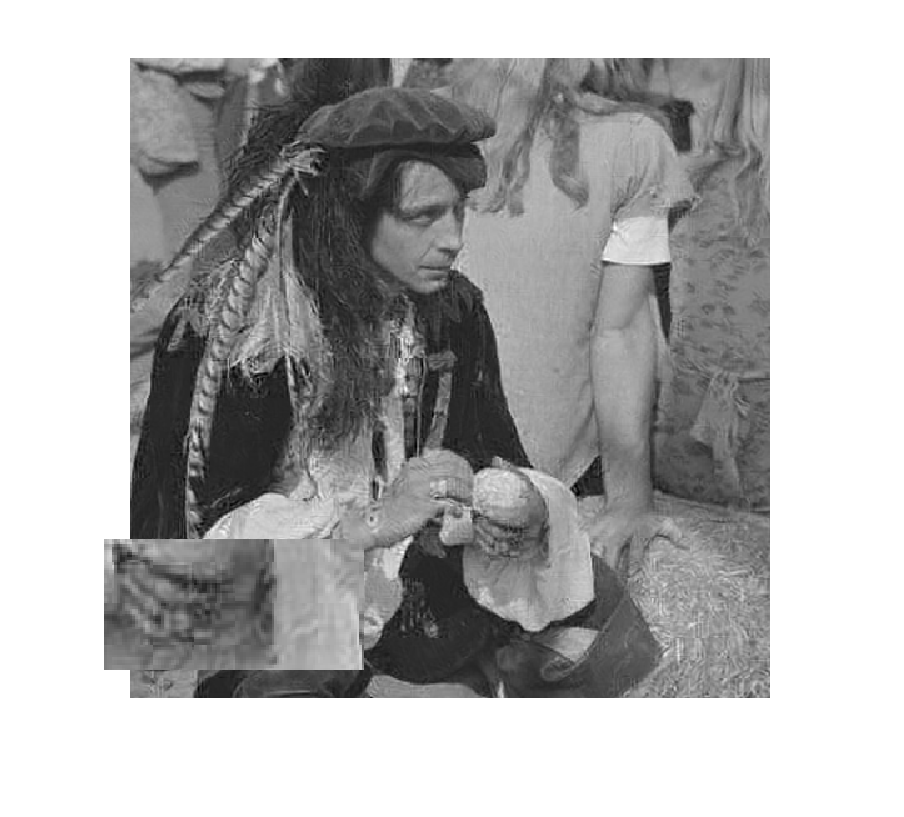
\includegraphics[width=.30\textwidth]{figChap4/Fig_pirate_hlzl.eps}}&
    \subfigure[$\text{CS}_{\text{HLZL}}$ with PSNR = $31.43$~dB]{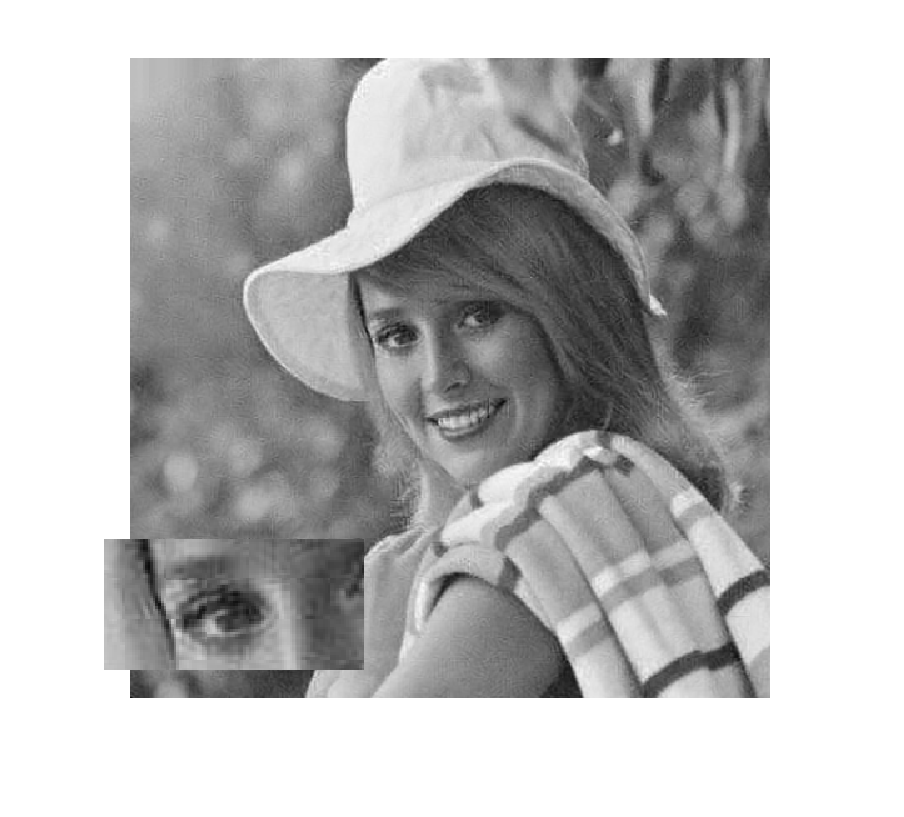
\includegraphics[width=.30\textwidth]{figChap4/Fig_elaine_hlzl.eps}}\\
    \subfigure[$\text{CS}_{\text{IR-PMD}}$ with PSNR = $34.18$~dB]{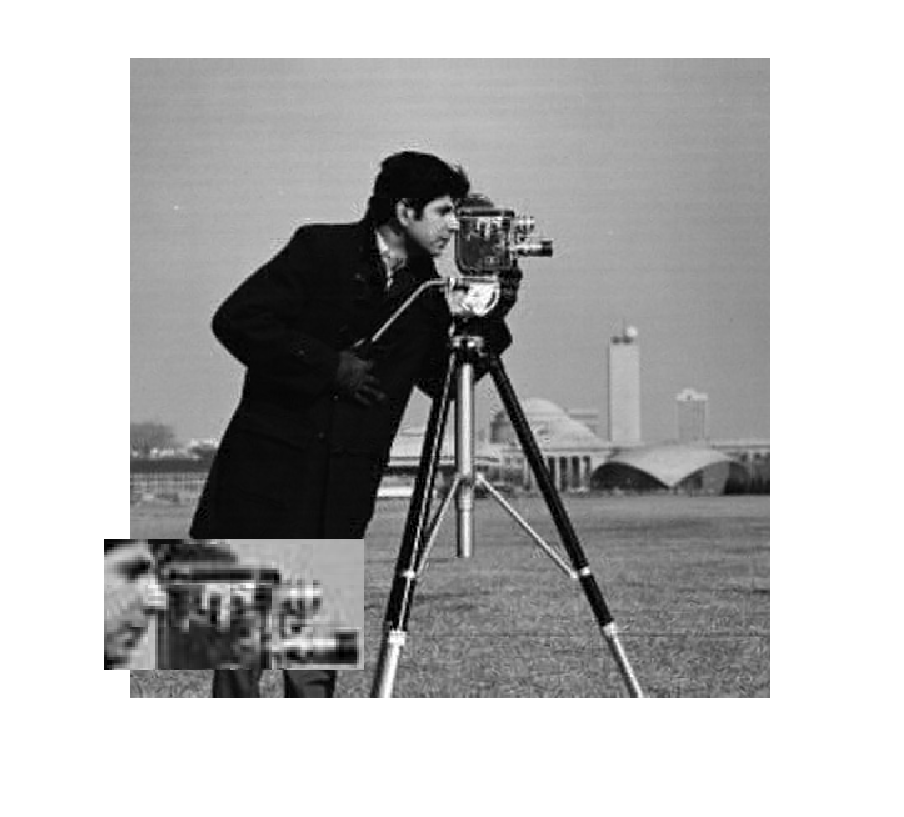
\includegraphics[width=.30\textwidth]{figChap4/Fig_Cam_21_camface_zoom.eps}} &
    \subfigure[$\text{CS}_{\text{IR-PMD}}$ with PSNR = $29.82$~dB]{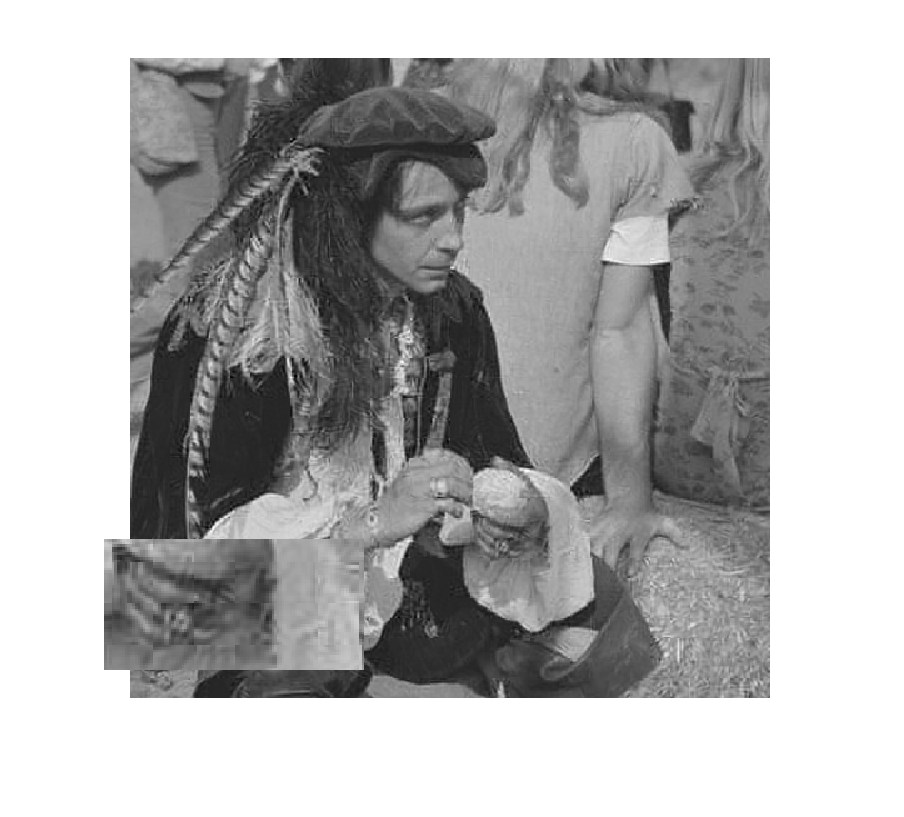
\includegraphics[width=.30\textwidth]{figChap4/Fig_pirate_21.eps}}&
    \subfigure[$\text{CS}_{\text{IR-PMD}}$ with PSNR = $32.29$~dB]{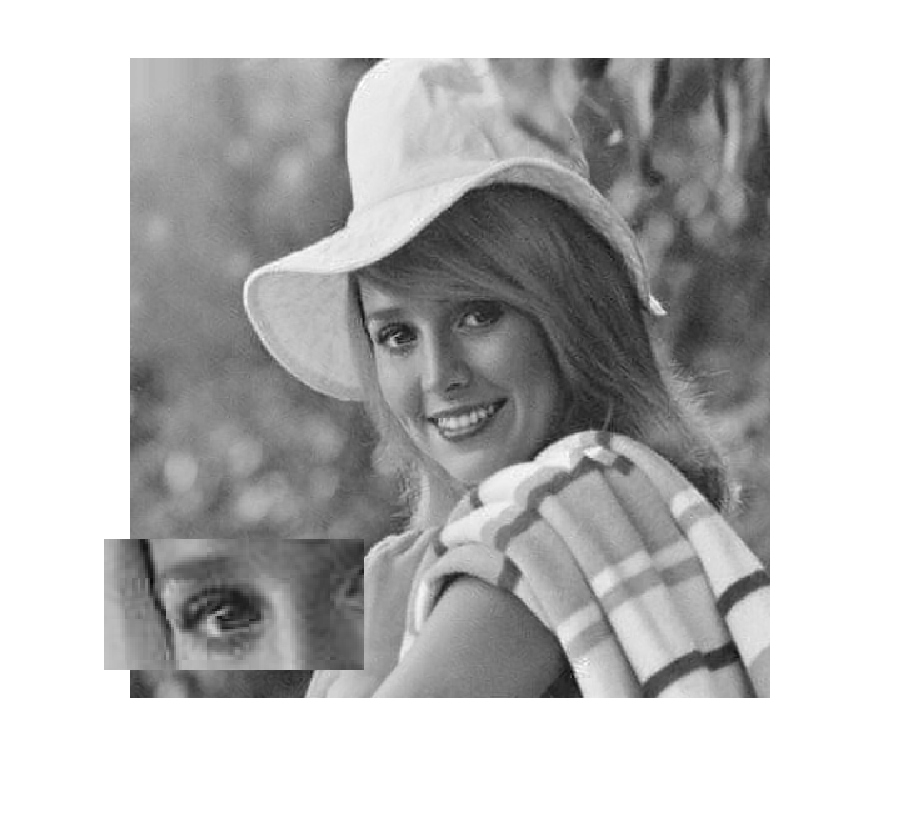
\includegraphics[width=.30\textwidth]{figChap4/Fig_elaine_21.eps}}\\
  \end{tabular}
\caption{Reconstruction performance on the standard \textit{Cameraman}, \textit{Pirate}, and \textit{Elaine} images with $M =80$, $s=16$, and $N=256$.}
  \label{Fig: Compare_Images}
\end{figure}
%
%
\begin{figure}
\centering    
\subfigure[Caltech-101 data set]{\label{fig:Comparison_cal }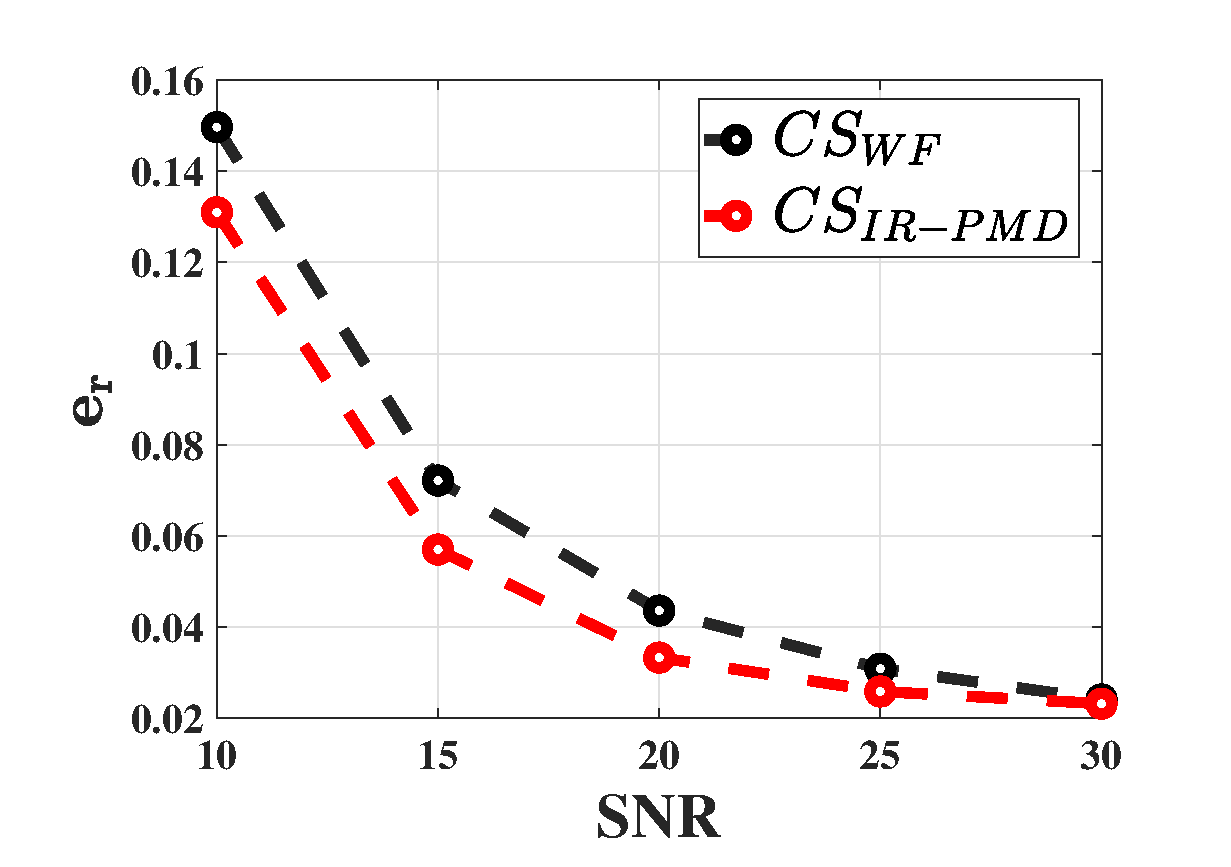
\includegraphics[keepaspectratio,width=0.43\textwidth,trim=17 0 0 0,clip]{figChap4/Comaprison_caltech.eps}}
\subfigure[Standard images]{\label{fig:Comparison_flowers}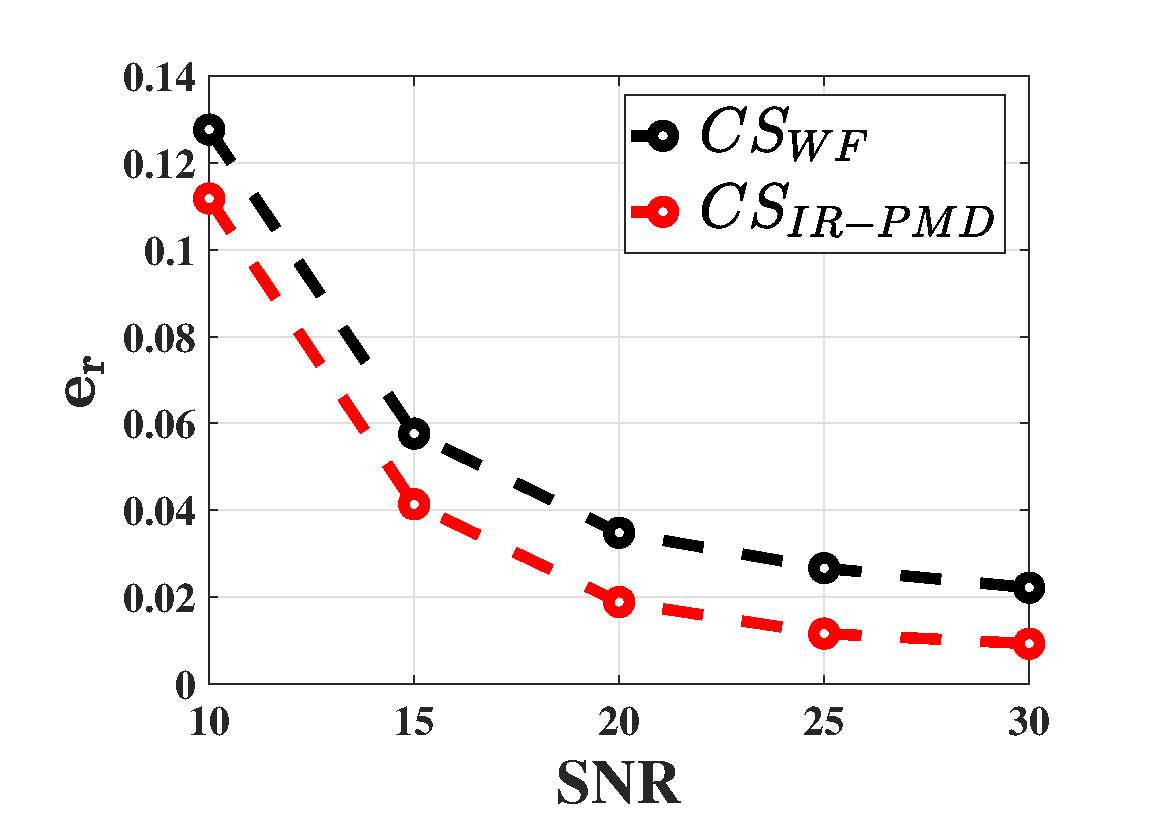
\includegraphics[keepaspectratio,width=0.43\textwidth,trim=17 0 0 0,clip]{figChap4/Comparison_std_mse.eps}} 
\caption{Comparison of the proposed IR-PMD method with the $\ell_{2,1}$ regularization and Frobenius norm regularization ($\text{CS}_{\text{WF}}$).}
\label{Fig Comparison_21_fro}
\end{figure}
%
%------------------------------------------------------%
\subsubsection{Caltech Data Set}
\label{subsec: Chap4_caltech_result}
%
In this experiment, we use the Caltech-101 data set~\cite{Caltech101} which contains a total of $9146$ images with $101$ different object categories and each object category has $40$-$800$ images. As in the previous experiment, these images are converted into training and testing patches. We obtain $60,000$ patches each of size $8 \times 8$ pixels with $50,000$ patches used for training and the remaining $10,000$ used for testing the recovery performance. The training data is used to train the sparsifying basis. For experiments with different values of SNR, $1000$ samples are randomly selected from $\bm{X}^{\text{train}}$ for each run. Then, white Gaussian noise is added to each subset of the training samples with SNR varying from $5$ dB to $45$ dB. The test data set $\bm{X}^{\text{test}}$ is divided into 10 testing subsets each with $1000$ samples which are used to evaluate recovery performance of the different CS systems over $1000$ trials. 

In Fig.~\ref{fig: PSNR_SNR_label}, the output PSNR is shown for SNR ranging from $5$ dB to $30$ dB. The results show that PSNR for $\text{CS}_{\text{IR-PMD}}$ is better than the other techniques. The performance of the mutual coherence-based methods is inferior to even $\text{CS}_{\text{rand}}$ when testing on real images with additional noise. The proposed method achieves improved performance compared to the sensing matrix design methods which take into account the SEE in their models such as~\cite{HONG_robust, HONG_sparse, SRE_Huang}, and is robust even at low SNRs, as the sensing matrix energy is minimized adaptively based on the reconstruction fidelity. %(\textcolor{blue}{With comparison to the state-of-the-art algorithms and from the pattern recognition-based literature, robustness is defined as the ability of the algorithm to perform w.r.t the data corruptions and outliers. In all experimental results of the proposed approach, the performance (PSNR, NMSE) doesn't fall greatly (does not changes a lot) with varying noise (for 10 dB, 20 dB and for real life images too).}) 
In Fig.~\ref{fig: NMSE_SNR_label}, MSE is shown as a function of SNR and $\text{CS}_{\text{IR-PMD}}$ achieves the best performance among the techniques being compared. Fig.~\ref{Fig: Compare_Images} compares the performance of $\text{CS}_{\text{HLZL}}$ and $\text{CS}_{\text{IR-PMD}}$ algorithms using a projection matrix $\bm{\Phi}$ trained at SNR $=5$~dB. Additional noise is not added to these images as real images already contain noise resulting in a sparse encoding error.
%---------------------------------------------------%
As seen in the inset zoom-in views, based on visual inspection, the edges are better recovered using $\text{CS}_{\text{IR-PMD}}$ along with improved visual quality of the images.
%The proposed method achieves the best qualitative results in these tests. 
Using the optimized projections designed by the IR-PMD algorithm, PSNR of the reconstructed images is higher than that of the images reconstructed using the other CS systems. Experimental results on synthetic data, real standard images, and the Caltech-101 data set have demonstrated the effectiveness of the proposed method.

Finally, in order to demonstrate the effectiveness of the $\ell_{2,1}$-norm regularization, we compare the performance of $\text{CS}_{\text{IR-PMD}}$ with $\text{CS}_{\text{WF}}$ which employs Frobenius norm and optimizes the objective $\| \bm{\Phi} \bm{\Psi} - \bm{D}_{ETF} \|_{F}^{2} + \gamma \| \bm{\Phi} \bm{E} \|_{F}^{2}$. The experimental settings and training-test data split for both Caltech-101 data set and standard images are kept the same as discussed in Section~\ref{subsec: Chap4_caltech_result}. Each of the experiments is repeated $1000$ times and the mean $e_r$ is reported. Fig.~\ref{Fig Comparison_21_fro} shows that $\text{CS}_{\text{IR-PMD}}$ based on the $\ell_{2,1}$-norm consistently performs better than the model based on the Frobenius norm.
%
\section{Chapter Summary}
%
In this chapter, we have proposed an algorithm for the design of incoherent and robust projection matrix as per the objectives discussed in Section~\ref{sec: Chap2_Mot_obj}. We have demonstrated that the $\ell_{2,1}$-norm leads to a more robust formulation while effectively minimizing the sensing matrix energy. In practice, the equivalent dictionary should be close to being a tight frame in order to achieve good recovery performance. In this work, we proposed a novel ETF design method based on the structural and spectral constraints on the eigenvalue characteristics. The resulting tight frame is used to design optimized projections. In addition to the mutual coherence and tightness constraints, the weighted sensing matrix energy term acts as a penalty to avoid amplification of the sparse encoding error in the measurement domain. A closed form solution set for an optimal sensing matrix with weighted penalty has been derived. Performance of the proposed algorithm is evaluated through extensive experiments on synthetic as well as real data.